\documentclass[11pt]{article}

    \usepackage[breakable]{tcolorbox}
    \usepackage{parskip} % Stop auto-indenting (to mimic markdown behaviour)
    
    \usepackage{iftex}
    \ifPDFTeX
    	\usepackage[T1]{fontenc}
    	\usepackage{mathpazo}
    \else
    	\usepackage{fontspec}
    \fi

    % Basic figure setup, for now with no caption control since it's done
    % automatically by Pandoc (which extracts ![](path) syntax from Markdown).
    \usepackage{graphicx}
    % Maintain compatibility with old templates. Remove in nbconvert 6.0
    \let\Oldincludegraphics\includegraphics
    % Ensure that by default, figures have no caption (until we provide a
    % proper Figure object with a Caption API and a way to capture that
    % in the conversion process - todo).
    \usepackage{caption}
    \DeclareCaptionFormat{nocaption}{}
    \captionsetup{format=nocaption,aboveskip=0pt,belowskip=0pt}

    \usepackage[Export]{adjustbox} % Used to constrain images to a maximum size
    \adjustboxset{max size={0.9\linewidth}{0.9\paperheight}}
    \usepackage{float}
    \floatplacement{figure}{H} % forces figures to be placed at the correct location
    \usepackage{xcolor} % Allow colors to be defined
    \usepackage{enumerate} % Needed for markdown enumerations to work
    \usepackage{geometry} % Used to adjust the document margins
    \usepackage{amsmath} % Equations
    \usepackage{amssymb} % Equations
    \usepackage{textcomp} % defines textquotesingle
    % Hack from http://tex.stackexchange.com/a/47451/13684:
    \AtBeginDocument{%
        \def\PYZsq{\textquotesingle}% Upright quotes in Pygmentized code
    }
    \usepackage{upquote} % Upright quotes for verbatim code
    \usepackage{eurosym} % defines \euro
    \usepackage[mathletters]{ucs} % Extended unicode (utf-8) support
    \usepackage{fancyvrb} % verbatim replacement that allows latex
    \usepackage{grffile} % extends the file name processing of package graphics 
                         % to support a larger range
    \makeatletter % fix for grffile with XeLaTeX
    \def\Gread@@xetex#1{%
      \IfFileExists{"\Gin@base".bb}%
      {\Gread@eps{\Gin@base.bb}}%
      {\Gread@@xetex@aux#1}%
    }
    \makeatother

    % The hyperref package gives us a pdf with properly built
    % internal navigation ('pdf bookmarks' for the table of contents,
    % internal cross-reference links, web links for URLs, etc.)
    \usepackage{hyperref}
    % The default LaTeX title has an obnoxious amount of whitespace. By default,
    % titling removes some of it. It also provides customization options.
    \usepackage{titling}
    \usepackage{longtable} % longtable support required by pandoc >1.10
    \usepackage{booktabs}  % table support for pandoc > 1.12.2
    \usepackage[inline]{enumitem} % IRkernel/repr support (it uses the enumerate* environment)
    \usepackage[normalem]{ulem} % ulem is needed to support strikethroughs (\sout)
                                % normalem makes italics be italics, not underlines
    \usepackage{mathrsfs}
    

    
    % Colors for the hyperref package
    \definecolor{urlcolor}{rgb}{0,.145,.698}
    \definecolor{linkcolor}{rgb}{.71,0.21,0.01}
    \definecolor{citecolor}{rgb}{.12,.54,.11}

    % ANSI colors
    \definecolor{ansi-black}{HTML}{3E424D}
    \definecolor{ansi-black-intense}{HTML}{282C36}
    \definecolor{ansi-red}{HTML}{E75C58}
    \definecolor{ansi-red-intense}{HTML}{B22B31}
    \definecolor{ansi-green}{HTML}{00A250}
    \definecolor{ansi-green-intense}{HTML}{007427}
    \definecolor{ansi-yellow}{HTML}{DDB62B}
    \definecolor{ansi-yellow-intense}{HTML}{B27D12}
    \definecolor{ansi-blue}{HTML}{208FFB}
    \definecolor{ansi-blue-intense}{HTML}{0065CA}
    \definecolor{ansi-magenta}{HTML}{D160C4}
    \definecolor{ansi-magenta-intense}{HTML}{A03196}
    \definecolor{ansi-cyan}{HTML}{60C6C8}
    \definecolor{ansi-cyan-intense}{HTML}{258F8F}
    \definecolor{ansi-white}{HTML}{C5C1B4}
    \definecolor{ansi-white-intense}{HTML}{A1A6B2}
    \definecolor{ansi-default-inverse-fg}{HTML}{FFFFFF}
    \definecolor{ansi-default-inverse-bg}{HTML}{000000}

    % commands and environments needed by pandoc snippets
    % extracted from the output of `pandoc -s`
    \providecommand{\tightlist}{%
      \setlength{\itemsep}{0pt}\setlength{\parskip}{0pt}}
    \DefineVerbatimEnvironment{Highlighting}{Verbatim}{commandchars=\\\{\}}
    % Add ',fontsize=\small' for more characters per line
    \newenvironment{Shaded}{}{}
    \newcommand{\KeywordTok}[1]{\textcolor[rgb]{0.00,0.44,0.13}{\textbf{{#1}}}}
    \newcommand{\DataTypeTok}[1]{\textcolor[rgb]{0.56,0.13,0.00}{{#1}}}
    \newcommand{\DecValTok}[1]{\textcolor[rgb]{0.25,0.63,0.44}{{#1}}}
    \newcommand{\BaseNTok}[1]{\textcolor[rgb]{0.25,0.63,0.44}{{#1}}}
    \newcommand{\FloatTok}[1]{\textcolor[rgb]{0.25,0.63,0.44}{{#1}}}
    \newcommand{\CharTok}[1]{\textcolor[rgb]{0.25,0.44,0.63}{{#1}}}
    \newcommand{\StringTok}[1]{\textcolor[rgb]{0.25,0.44,0.63}{{#1}}}
    \newcommand{\CommentTok}[1]{\textcolor[rgb]{0.38,0.63,0.69}{\textit{{#1}}}}
    \newcommand{\OtherTok}[1]{\textcolor[rgb]{0.00,0.44,0.13}{{#1}}}
    \newcommand{\AlertTok}[1]{\textcolor[rgb]{1.00,0.00,0.00}{\textbf{{#1}}}}
    \newcommand{\FunctionTok}[1]{\textcolor[rgb]{0.02,0.16,0.49}{{#1}}}
    \newcommand{\RegionMarkerTok}[1]{{#1}}
    \newcommand{\ErrorTok}[1]{\textcolor[rgb]{1.00,0.00,0.00}{\textbf{{#1}}}}
    \newcommand{\NormalTok}[1]{{#1}}
    
    % Additional commands for more recent versions of Pandoc
    \newcommand{\ConstantTok}[1]{\textcolor[rgb]{0.53,0.00,0.00}{{#1}}}
    \newcommand{\SpecialCharTok}[1]{\textcolor[rgb]{0.25,0.44,0.63}{{#1}}}
    \newcommand{\VerbatimStringTok}[1]{\textcolor[rgb]{0.25,0.44,0.63}{{#1}}}
    \newcommand{\SpecialStringTok}[1]{\textcolor[rgb]{0.73,0.40,0.53}{{#1}}}
    \newcommand{\ImportTok}[1]{{#1}}
    \newcommand{\DocumentationTok}[1]{\textcolor[rgb]{0.73,0.13,0.13}{\textit{{#1}}}}
    \newcommand{\AnnotationTok}[1]{\textcolor[rgb]{0.38,0.63,0.69}{\textbf{\textit{{#1}}}}}
    \newcommand{\CommentVarTok}[1]{\textcolor[rgb]{0.38,0.63,0.69}{\textbf{\textit{{#1}}}}}
    \newcommand{\VariableTok}[1]{\textcolor[rgb]{0.10,0.09,0.49}{{#1}}}
    \newcommand{\ControlFlowTok}[1]{\textcolor[rgb]{0.00,0.44,0.13}{\textbf{{#1}}}}
    \newcommand{\OperatorTok}[1]{\textcolor[rgb]{0.40,0.40,0.40}{{#1}}}
    \newcommand{\BuiltInTok}[1]{{#1}}
    \newcommand{\ExtensionTok}[1]{{#1}}
    \newcommand{\PreprocessorTok}[1]{\textcolor[rgb]{0.74,0.48,0.00}{{#1}}}
    \newcommand{\AttributeTok}[1]{\textcolor[rgb]{0.49,0.56,0.16}{{#1}}}
    \newcommand{\InformationTok}[1]{\textcolor[rgb]{0.38,0.63,0.69}{\textbf{\textit{{#1}}}}}
    \newcommand{\WarningTok}[1]{\textcolor[rgb]{0.38,0.63,0.69}{\textbf{\textit{{#1}}}}}
    
    
    % Define a nice break command that doesn't care if a line doesn't already
    % exist.
    \def\br{\hspace*{\fill} \\* }
    % Math Jax compatibility definitions
    \def\gt{>}
    \def\lt{<}
    \let\Oldtex\TeX
    \let\Oldlatex\LaTeX
    \renewcommand{\TeX}{\textrm{\Oldtex}}
    \renewcommand{\LaTeX}{\textrm{\Oldlatex}}
    % Document parameters
    % Document title
    \title{2021\_01\_06\_EE538\_Lecture1\_W2021}
    
    
    
    
    
% Pygments definitions
\makeatletter
\def\PY@reset{\let\PY@it=\relax \let\PY@bf=\relax%
    \let\PY@ul=\relax \let\PY@tc=\relax%
    \let\PY@bc=\relax \let\PY@ff=\relax}
\def\PY@tok#1{\csname PY@tok@#1\endcsname}
\def\PY@toks#1+{\ifx\relax#1\empty\else%
    \PY@tok{#1}\expandafter\PY@toks\fi}
\def\PY@do#1{\PY@bc{\PY@tc{\PY@ul{%
    \PY@it{\PY@bf{\PY@ff{#1}}}}}}}
\def\PY#1#2{\PY@reset\PY@toks#1+\relax+\PY@do{#2}}

\expandafter\def\csname PY@tok@w\endcsname{\def\PY@tc##1{\textcolor[rgb]{0.73,0.73,0.73}{##1}}}
\expandafter\def\csname PY@tok@c\endcsname{\let\PY@it=\textit\def\PY@tc##1{\textcolor[rgb]{0.25,0.50,0.50}{##1}}}
\expandafter\def\csname PY@tok@cp\endcsname{\def\PY@tc##1{\textcolor[rgb]{0.74,0.48,0.00}{##1}}}
\expandafter\def\csname PY@tok@k\endcsname{\let\PY@bf=\textbf\def\PY@tc##1{\textcolor[rgb]{0.00,0.50,0.00}{##1}}}
\expandafter\def\csname PY@tok@kp\endcsname{\def\PY@tc##1{\textcolor[rgb]{0.00,0.50,0.00}{##1}}}
\expandafter\def\csname PY@tok@kt\endcsname{\def\PY@tc##1{\textcolor[rgb]{0.69,0.00,0.25}{##1}}}
\expandafter\def\csname PY@tok@o\endcsname{\def\PY@tc##1{\textcolor[rgb]{0.40,0.40,0.40}{##1}}}
\expandafter\def\csname PY@tok@ow\endcsname{\let\PY@bf=\textbf\def\PY@tc##1{\textcolor[rgb]{0.67,0.13,1.00}{##1}}}
\expandafter\def\csname PY@tok@nb\endcsname{\def\PY@tc##1{\textcolor[rgb]{0.00,0.50,0.00}{##1}}}
\expandafter\def\csname PY@tok@nf\endcsname{\def\PY@tc##1{\textcolor[rgb]{0.00,0.00,1.00}{##1}}}
\expandafter\def\csname PY@tok@nc\endcsname{\let\PY@bf=\textbf\def\PY@tc##1{\textcolor[rgb]{0.00,0.00,1.00}{##1}}}
\expandafter\def\csname PY@tok@nn\endcsname{\let\PY@bf=\textbf\def\PY@tc##1{\textcolor[rgb]{0.00,0.00,1.00}{##1}}}
\expandafter\def\csname PY@tok@ne\endcsname{\let\PY@bf=\textbf\def\PY@tc##1{\textcolor[rgb]{0.82,0.25,0.23}{##1}}}
\expandafter\def\csname PY@tok@nv\endcsname{\def\PY@tc##1{\textcolor[rgb]{0.10,0.09,0.49}{##1}}}
\expandafter\def\csname PY@tok@no\endcsname{\def\PY@tc##1{\textcolor[rgb]{0.53,0.00,0.00}{##1}}}
\expandafter\def\csname PY@tok@nl\endcsname{\def\PY@tc##1{\textcolor[rgb]{0.63,0.63,0.00}{##1}}}
\expandafter\def\csname PY@tok@ni\endcsname{\let\PY@bf=\textbf\def\PY@tc##1{\textcolor[rgb]{0.60,0.60,0.60}{##1}}}
\expandafter\def\csname PY@tok@na\endcsname{\def\PY@tc##1{\textcolor[rgb]{0.49,0.56,0.16}{##1}}}
\expandafter\def\csname PY@tok@nt\endcsname{\let\PY@bf=\textbf\def\PY@tc##1{\textcolor[rgb]{0.00,0.50,0.00}{##1}}}
\expandafter\def\csname PY@tok@nd\endcsname{\def\PY@tc##1{\textcolor[rgb]{0.67,0.13,1.00}{##1}}}
\expandafter\def\csname PY@tok@s\endcsname{\def\PY@tc##1{\textcolor[rgb]{0.73,0.13,0.13}{##1}}}
\expandafter\def\csname PY@tok@sd\endcsname{\let\PY@it=\textit\def\PY@tc##1{\textcolor[rgb]{0.73,0.13,0.13}{##1}}}
\expandafter\def\csname PY@tok@si\endcsname{\let\PY@bf=\textbf\def\PY@tc##1{\textcolor[rgb]{0.73,0.40,0.53}{##1}}}
\expandafter\def\csname PY@tok@se\endcsname{\let\PY@bf=\textbf\def\PY@tc##1{\textcolor[rgb]{0.73,0.40,0.13}{##1}}}
\expandafter\def\csname PY@tok@sr\endcsname{\def\PY@tc##1{\textcolor[rgb]{0.73,0.40,0.53}{##1}}}
\expandafter\def\csname PY@tok@ss\endcsname{\def\PY@tc##1{\textcolor[rgb]{0.10,0.09,0.49}{##1}}}
\expandafter\def\csname PY@tok@sx\endcsname{\def\PY@tc##1{\textcolor[rgb]{0.00,0.50,0.00}{##1}}}
\expandafter\def\csname PY@tok@m\endcsname{\def\PY@tc##1{\textcolor[rgb]{0.40,0.40,0.40}{##1}}}
\expandafter\def\csname PY@tok@gh\endcsname{\let\PY@bf=\textbf\def\PY@tc##1{\textcolor[rgb]{0.00,0.00,0.50}{##1}}}
\expandafter\def\csname PY@tok@gu\endcsname{\let\PY@bf=\textbf\def\PY@tc##1{\textcolor[rgb]{0.50,0.00,0.50}{##1}}}
\expandafter\def\csname PY@tok@gd\endcsname{\def\PY@tc##1{\textcolor[rgb]{0.63,0.00,0.00}{##1}}}
\expandafter\def\csname PY@tok@gi\endcsname{\def\PY@tc##1{\textcolor[rgb]{0.00,0.63,0.00}{##1}}}
\expandafter\def\csname PY@tok@gr\endcsname{\def\PY@tc##1{\textcolor[rgb]{1.00,0.00,0.00}{##1}}}
\expandafter\def\csname PY@tok@ge\endcsname{\let\PY@it=\textit}
\expandafter\def\csname PY@tok@gs\endcsname{\let\PY@bf=\textbf}
\expandafter\def\csname PY@tok@gp\endcsname{\let\PY@bf=\textbf\def\PY@tc##1{\textcolor[rgb]{0.00,0.00,0.50}{##1}}}
\expandafter\def\csname PY@tok@go\endcsname{\def\PY@tc##1{\textcolor[rgb]{0.53,0.53,0.53}{##1}}}
\expandafter\def\csname PY@tok@gt\endcsname{\def\PY@tc##1{\textcolor[rgb]{0.00,0.27,0.87}{##1}}}
\expandafter\def\csname PY@tok@err\endcsname{\def\PY@bc##1{\setlength{\fboxsep}{0pt}\fcolorbox[rgb]{1.00,0.00,0.00}{1,1,1}{\strut ##1}}}
\expandafter\def\csname PY@tok@kc\endcsname{\let\PY@bf=\textbf\def\PY@tc##1{\textcolor[rgb]{0.00,0.50,0.00}{##1}}}
\expandafter\def\csname PY@tok@kd\endcsname{\let\PY@bf=\textbf\def\PY@tc##1{\textcolor[rgb]{0.00,0.50,0.00}{##1}}}
\expandafter\def\csname PY@tok@kn\endcsname{\let\PY@bf=\textbf\def\PY@tc##1{\textcolor[rgb]{0.00,0.50,0.00}{##1}}}
\expandafter\def\csname PY@tok@kr\endcsname{\let\PY@bf=\textbf\def\PY@tc##1{\textcolor[rgb]{0.00,0.50,0.00}{##1}}}
\expandafter\def\csname PY@tok@bp\endcsname{\def\PY@tc##1{\textcolor[rgb]{0.00,0.50,0.00}{##1}}}
\expandafter\def\csname PY@tok@fm\endcsname{\def\PY@tc##1{\textcolor[rgb]{0.00,0.00,1.00}{##1}}}
\expandafter\def\csname PY@tok@vc\endcsname{\def\PY@tc##1{\textcolor[rgb]{0.10,0.09,0.49}{##1}}}
\expandafter\def\csname PY@tok@vg\endcsname{\def\PY@tc##1{\textcolor[rgb]{0.10,0.09,0.49}{##1}}}
\expandafter\def\csname PY@tok@vi\endcsname{\def\PY@tc##1{\textcolor[rgb]{0.10,0.09,0.49}{##1}}}
\expandafter\def\csname PY@tok@vm\endcsname{\def\PY@tc##1{\textcolor[rgb]{0.10,0.09,0.49}{##1}}}
\expandafter\def\csname PY@tok@sa\endcsname{\def\PY@tc##1{\textcolor[rgb]{0.73,0.13,0.13}{##1}}}
\expandafter\def\csname PY@tok@sb\endcsname{\def\PY@tc##1{\textcolor[rgb]{0.73,0.13,0.13}{##1}}}
\expandafter\def\csname PY@tok@sc\endcsname{\def\PY@tc##1{\textcolor[rgb]{0.73,0.13,0.13}{##1}}}
\expandafter\def\csname PY@tok@dl\endcsname{\def\PY@tc##1{\textcolor[rgb]{0.73,0.13,0.13}{##1}}}
\expandafter\def\csname PY@tok@s2\endcsname{\def\PY@tc##1{\textcolor[rgb]{0.73,0.13,0.13}{##1}}}
\expandafter\def\csname PY@tok@sh\endcsname{\def\PY@tc##1{\textcolor[rgb]{0.73,0.13,0.13}{##1}}}
\expandafter\def\csname PY@tok@s1\endcsname{\def\PY@tc##1{\textcolor[rgb]{0.73,0.13,0.13}{##1}}}
\expandafter\def\csname PY@tok@mb\endcsname{\def\PY@tc##1{\textcolor[rgb]{0.40,0.40,0.40}{##1}}}
\expandafter\def\csname PY@tok@mf\endcsname{\def\PY@tc##1{\textcolor[rgb]{0.40,0.40,0.40}{##1}}}
\expandafter\def\csname PY@tok@mh\endcsname{\def\PY@tc##1{\textcolor[rgb]{0.40,0.40,0.40}{##1}}}
\expandafter\def\csname PY@tok@mi\endcsname{\def\PY@tc##1{\textcolor[rgb]{0.40,0.40,0.40}{##1}}}
\expandafter\def\csname PY@tok@il\endcsname{\def\PY@tc##1{\textcolor[rgb]{0.40,0.40,0.40}{##1}}}
\expandafter\def\csname PY@tok@mo\endcsname{\def\PY@tc##1{\textcolor[rgb]{0.40,0.40,0.40}{##1}}}
\expandafter\def\csname PY@tok@ch\endcsname{\let\PY@it=\textit\def\PY@tc##1{\textcolor[rgb]{0.25,0.50,0.50}{##1}}}
\expandafter\def\csname PY@tok@cm\endcsname{\let\PY@it=\textit\def\PY@tc##1{\textcolor[rgb]{0.25,0.50,0.50}{##1}}}
\expandafter\def\csname PY@tok@cpf\endcsname{\let\PY@it=\textit\def\PY@tc##1{\textcolor[rgb]{0.25,0.50,0.50}{##1}}}
\expandafter\def\csname PY@tok@c1\endcsname{\let\PY@it=\textit\def\PY@tc##1{\textcolor[rgb]{0.25,0.50,0.50}{##1}}}
\expandafter\def\csname PY@tok@cs\endcsname{\let\PY@it=\textit\def\PY@tc##1{\textcolor[rgb]{0.25,0.50,0.50}{##1}}}

\def\PYZbs{\char`\\}
\def\PYZus{\char`\_}
\def\PYZob{\char`\{}
\def\PYZcb{\char`\}}
\def\PYZca{\char`\^}
\def\PYZam{\char`\&}
\def\PYZlt{\char`\<}
\def\PYZgt{\char`\>}
\def\PYZsh{\char`\#}
\def\PYZpc{\char`\%}
\def\PYZdl{\char`\$}
\def\PYZhy{\char`\-}
\def\PYZsq{\char`\'}
\def\PYZdq{\char`\"}
\def\PYZti{\char`\~}
% for compatibility with earlier versions
\def\PYZat{@}
\def\PYZlb{[}
\def\PYZrb{]}
\makeatother


    % For linebreaks inside Verbatim environment from package fancyvrb. 
    \makeatletter
        \newbox\Wrappedcontinuationbox 
        \newbox\Wrappedvisiblespacebox 
        \newcommand*\Wrappedvisiblespace {\textcolor{red}{\textvisiblespace}} 
        \newcommand*\Wrappedcontinuationsymbol {\textcolor{red}{\llap{\tiny$\m@th\hookrightarrow$}}} 
        \newcommand*\Wrappedcontinuationindent {3ex } 
        \newcommand*\Wrappedafterbreak {\kern\Wrappedcontinuationindent\copy\Wrappedcontinuationbox} 
        % Take advantage of the already applied Pygments mark-up to insert 
        % potential linebreaks for TeX processing. 
        %        {, <, #, %, $, ' and ": go to next line. 
        %        _, }, ^, &, >, - and ~: stay at end of broken line. 
        % Use of \textquotesingle for straight quote. 
        \newcommand*\Wrappedbreaksatspecials {% 
            \def\PYGZus{\discretionary{\char`\_}{\Wrappedafterbreak}{\char`\_}}% 
            \def\PYGZob{\discretionary{}{\Wrappedafterbreak\char`\{}{\char`\{}}% 
            \def\PYGZcb{\discretionary{\char`\}}{\Wrappedafterbreak}{\char`\}}}% 
            \def\PYGZca{\discretionary{\char`\^}{\Wrappedafterbreak}{\char`\^}}% 
            \def\PYGZam{\discretionary{\char`\&}{\Wrappedafterbreak}{\char`\&}}% 
            \def\PYGZlt{\discretionary{}{\Wrappedafterbreak\char`\<}{\char`\<}}% 
            \def\PYGZgt{\discretionary{\char`\>}{\Wrappedafterbreak}{\char`\>}}% 
            \def\PYGZsh{\discretionary{}{\Wrappedafterbreak\char`\#}{\char`\#}}% 
            \def\PYGZpc{\discretionary{}{\Wrappedafterbreak\char`\%}{\char`\%}}% 
            \def\PYGZdl{\discretionary{}{\Wrappedafterbreak\char`\$}{\char`\$}}% 
            \def\PYGZhy{\discretionary{\char`\-}{\Wrappedafterbreak}{\char`\-}}% 
            \def\PYGZsq{\discretionary{}{\Wrappedafterbreak\textquotesingle}{\textquotesingle}}% 
            \def\PYGZdq{\discretionary{}{\Wrappedafterbreak\char`\"}{\char`\"}}% 
            \def\PYGZti{\discretionary{\char`\~}{\Wrappedafterbreak}{\char`\~}}% 
        } 
        % Some characters . , ; ? ! / are not pygmentized. 
        % This macro makes them "active" and they will insert potential linebreaks 
        \newcommand*\Wrappedbreaksatpunct {% 
            \lccode`\~`\.\lowercase{\def~}{\discretionary{\hbox{\char`\.}}{\Wrappedafterbreak}{\hbox{\char`\.}}}% 
            \lccode`\~`\,\lowercase{\def~}{\discretionary{\hbox{\char`\,}}{\Wrappedafterbreak}{\hbox{\char`\,}}}% 
            \lccode`\~`\;\lowercase{\def~}{\discretionary{\hbox{\char`\;}}{\Wrappedafterbreak}{\hbox{\char`\;}}}% 
            \lccode`\~`\:\lowercase{\def~}{\discretionary{\hbox{\char`\:}}{\Wrappedafterbreak}{\hbox{\char`\:}}}% 
            \lccode`\~`\?\lowercase{\def~}{\discretionary{\hbox{\char`\?}}{\Wrappedafterbreak}{\hbox{\char`\?}}}% 
            \lccode`\~`\!\lowercase{\def~}{\discretionary{\hbox{\char`\!}}{\Wrappedafterbreak}{\hbox{\char`\!}}}% 
            \lccode`\~`\/\lowercase{\def~}{\discretionary{\hbox{\char`\/}}{\Wrappedafterbreak}{\hbox{\char`\/}}}% 
            \catcode`\.\active
            \catcode`\,\active 
            \catcode`\;\active
            \catcode`\:\active
            \catcode`\?\active
            \catcode`\!\active
            \catcode`\/\active 
            \lccode`\~`\~ 	
        }
    \makeatother

    \let\OriginalVerbatim=\Verbatim
    \makeatletter
    \renewcommand{\Verbatim}[1][1]{%
        %\parskip\z@skip
        \sbox\Wrappedcontinuationbox {\Wrappedcontinuationsymbol}%
        \sbox\Wrappedvisiblespacebox {\FV@SetupFont\Wrappedvisiblespace}%
        \def\FancyVerbFormatLine ##1{\hsize\linewidth
            \vtop{\raggedright\hyphenpenalty\z@\exhyphenpenalty\z@
                \doublehyphendemerits\z@\finalhyphendemerits\z@
                \strut ##1\strut}%
        }%
        % If the linebreak is at a space, the latter will be displayed as visible
        % space at end of first line, and a continuation symbol starts next line.
        % Stretch/shrink are however usually zero for typewriter font.
        \def\FV@Space {%
            \nobreak\hskip\z@ plus\fontdimen3\font minus\fontdimen4\font
            \discretionary{\copy\Wrappedvisiblespacebox}{\Wrappedafterbreak}
            {\kern\fontdimen2\font}%
        }%
        
        % Allow breaks at special characters using \PYG... macros.
        \Wrappedbreaksatspecials
        % Breaks at punctuation characters . , ; ? ! and / need catcode=\active 	
        \OriginalVerbatim[#1,codes*=\Wrappedbreaksatpunct]%
    }
    \makeatother

    % Exact colors from NB
    \definecolor{incolor}{HTML}{303F9F}
    \definecolor{outcolor}{HTML}{D84315}
    \definecolor{cellborder}{HTML}{CFCFCF}
    \definecolor{cellbackground}{HTML}{F7F7F7}
    
    % prompt
    \makeatletter
    \newcommand{\boxspacing}{\kern\kvtcb@left@rule\kern\kvtcb@boxsep}
    \makeatother
    \newcommand{\prompt}[4]{
        \ttfamily\llap{{\color{#2}[#3]:\hspace{3pt}#4}}\vspace{-\baselineskip}
    }
    

    
    % Prevent overflowing lines due to hard-to-break entities
    \sloppy 
    % Setup hyperref package
    \hypersetup{
      breaklinks=true,  % so long urls are correctly broken across lines
      colorlinks=true,
      urlcolor=urlcolor,
      linkcolor=linkcolor,
      citecolor=citecolor,
      }
    % Slightly bigger margins than the latex defaults
    
    \geometry{verbose,tmargin=1in,bmargin=1in,lmargin=1in,rmargin=1in}
    
    

\begin{document}
    
    \maketitle
    
    

    
    \hypertarget{ee-538-analog-integrated-circuit-design}{%
\section{EE 538: Analog Integrated Circuit
Design}\label{ee-538-analog-integrated-circuit-design}}

\hypertarget{winter-2021}{%
\subsection{Winter 2021}\label{winter-2021}}

\hypertarget{instructor-jason-silver}{%
\subsection{Instructor: Jason Silver}\label{instructor-jason-silver}}

    \hypertarget{ee-538-basics-i}{%
\subsection{EE 538 basics I}\label{ee-538-basics-i}}

    \begin{itemize}
\tightlist
\item
  Instructor

  \begin{itemize}
  \tightlist
  \item
    Jason Silver
  \item
    Office hours TBD via Google poll
  \end{itemize}
\item
  Teaching assistant

  \begin{itemize}
  \tightlist
  \item
    Thushara Maria Xavier
  \item
    Office hours TBD
  \end{itemize}
\item
  Web page: \href{https://canvas.uw.edu/courses/1448967}{EE 538 Winter
  2021 (Canvas)}

  \begin{itemize}
  \tightlist
  \item
    Access assignments, grades, and solutions
  \end{itemize}
\item
  Slack

  \begin{itemize}
  \tightlist
  \item
    \href{https://join.slack.com/t/uwaic2021/shared_invite/zt-k8e4c07p-6mkI7JSqfLv_lYJ21zW2ZQ}{EE
    538 Winter 2021 Slack workspace}
  \item
    Use Slack to ask questions about assignments and projects
  \item
    Participation in online discussion benefits everyone!
  \end{itemize}
\end{itemize}

    \hypertarget{ee-538-basics-ii}{%
\subsection{EE 538 basics II}\label{ee-538-basics-ii}}

    \begin{itemize}
\tightlist
\item
  There are no official prerequisites, but it will be helpful to have
  some familiarity with

  \begin{itemize}
  \tightlist
  \item
    Elementary circuit theory

    \begin{itemize}
    \tightlist
    \item
      KVL, KCL, Thevenin equivalent circuits, Laplace/Fourier transforms
    \end{itemize}
  \item
    Semiconductor device operation and circuit analysis

    \begin{itemize}
    \tightlist
    \item
      Diodes, FETs, BJTs
    \end{itemize}
  \item
    Basic linear systems

    \begin{itemize}
    \tightlist
    \item
      Frequency response, poles, zeros, Bode plots
    \end{itemize}
  \item
    Circuit simulation with some flavor of SPICE (\_\_S\_\_imulation
    \_\_P\_\_rogram with \_\_I\_\_ntegrated \_\_C\_\_ircuit
    \_\_E\_\_mphasis)
  \end{itemize}
\end{itemize}

    \hypertarget{about-your-instructor}{%
\subsection{About your instructor}\label{about-your-instructor}}

    \begin{itemize}
\tightlist
\item
  PhD from UW EE in 2015

  \begin{itemize}
  \tightlist
  \item
    Low power integrated circuit (IC) design for bioelectrical
    interfaces

    \begin{itemize}
    \tightlist
    \item
      EEG, EMG, neural recording
    \end{itemize}
  \item
    Focus on optimizing for power efficiency
  \end{itemize}
\item
  13 years experience designing ICs and systems for academia and
  industry

  \begin{itemize}
  \tightlist
  \item
    Mixed-signal design for biomedical applications
  \end{itemize}
\item
  Current full-time role

  \begin{itemize}
  \tightlist
  \item
    Director of Hardware and Biosystems Engineering at Curi Bio

    \begin{itemize}
    \tightlist
    \item
      Formerly housed in UW CoMotion startup incubator (Fluke Hall)
    \item
      Instrumentation for \emph{in vitro} cell studies
    \end{itemize}
  \end{itemize}
\end{itemize}

    \hypertarget{course-breakdown}{%
\subsection{Course breakdown}\label{course-breakdown}}

    \begin{itemize}
\tightlist
\item
  Weekly Assignments (40\%)

  \begin{itemize}
  \tightlist
  \item
    Typically assigned Saturday, submitted online the Sunday of the
    following week
  \end{itemize}
\item
  Design project (40\%)

  \begin{itemize}
  \tightlist
  \item
    Analog IC design project using Cadence tools
  \item
    Optimization for performance, power, cost
  \end{itemize}
\item
  Midterm exam (20\%)

  \begin{itemize}
  \tightlist
  \item
    Single exam covering approximately half of the course material
  \item
    ``Take-home'' format, submitted online
  \end{itemize}
\end{itemize}

    \hypertarget{course-learning-goals}{%
\subsection{Course learning goals}\label{course-learning-goals}}

    \begin{itemize}
\tightlist
\item
  Develop deeper understanding of MOS transistor behavior relevant to
  analog (and some digital) design
\item
  Develop intuition w.r.t. tradeoffs in analog circuits (speed, noise,
  power dissipation)
\item
  Learn to bridge the gap between complex device models/behavior and
  ``back-of-the-envelope'' calculations
\item
  Develop a systematic approach to circuit analysis and design
\end{itemize}

    \hypertarget{course-topics}{%
\subsection{Course topics}\label{course-topics}}

    \begin{itemize}
\tightlist
\item
  CMOS technology and device models
\item
  Single-stage amplifiers
\item
  Current mirrors, active loads
\item
  Differential pairs
\item
  Operational transconductance amplifiers (OTAs)
\item
  Feedback, stability, and compensation
\end{itemize}

    \hypertarget{software-and-cad}{%
\subsection{Software and CAD}\label{software-and-cad}}

    \begin{itemize}
\tightlist
\item
  We will use Cadence for circuit simulation

  \begin{itemize}
  \tightlist
  \item
    Tutorial following today's lecture
  \end{itemize}
\item
  Design, data analysis, and results plotting using Python/Jupyter
  Notebooks

  \begin{itemize}
  \tightlist
  \item
    Design scripts iterable and reusable
  \item
    More flexible than Cadence native plotting functions
  \item
    Lecture examples created using Python/Jupyter Notebooks
  \end{itemize}
\end{itemize}

    \hypertarget{spice-design-methodology}{%
\subsection{SPICE design methodology}\label{spice-design-methodology}}

    \begin{itemize}
\tightlist
\item
  SPICE is a numerical simulation tool that enables you to evaluate
  circuit ideas
\item
  General rule: Don't simulate something you don't already (mostly)
  understand

  \begin{itemize}
  \tightlist
  \item
    SPICE is for verification only!
  \end{itemize}
\item
  Neither analytical nor simulation models provide a complete picture of
  reality

  \begin{itemize}
  \tightlist
  \item
    Understanding model limitations is crucial to building successful
    circuits and systems
  \end{itemize}
\end{itemize}

    \hypertarget{jupyterhub}{%
\subsection{JupyterHub}\label{jupyterhub}}

    \begin{itemize}
\tightlist
\item
  Jupyter Hub enables execution of Python code without the need for
  installation/maintenance of packages, etc
\item
  Lecture notes/slides will be made available in student directories
  several days prior to lecture
\item
  \href{https://rttl.axdd.s.uw.edu/2021-winter-e-e-538-c}{EE538 Jupyter
  Hub Server}
\item
  Please log out of the server when you're not using it!
\end{itemize}

    \hypertarget{python-packagesmodules}{%
\subsection{Python packages/modules}\label{python-packagesmodules}}

    \begin{tcolorbox}[breakable, size=fbox, boxrule=1pt, pad at break*=1mm,colback=cellbackground, colframe=cellborder]
\prompt{In}{incolor}{2}{\boxspacing}
\begin{Verbatim}[commandchars=\\\{\}]
\PY{k+kn}{import} \PY{n+nn}{matplotlib} \PY{k}{as} \PY{n+nn}{mpl}
\PY{k+kn}{from} \PY{n+nn}{matplotlib} \PY{k+kn}{import} \PY{n}{pyplot} \PY{k}{as} \PY{n}{plt}
\PY{k+kn}{import} \PY{n+nn}{numpy} \PY{k}{as} \PY{n+nn}{np}
\PY{k+kn}{from} \PY{n+nn}{scipy} \PY{k+kn}{import} \PY{n}{signal}
\PY{c+c1}{\PYZsh{}\PYZpc{}matplotlib notebook}

\PY{n}{mpl}\PY{o}{.}\PY{n}{rcParams}\PY{p}{[}\PY{l+s+s1}{\PYZsq{}}\PY{l+s+s1}{font.size}\PY{l+s+s1}{\PYZsq{}}\PY{p}{]} \PY{o}{=} \PY{l+m+mi}{12}
\PY{n}{mpl}\PY{o}{.}\PY{n}{rcParams}\PY{p}{[}\PY{l+s+s1}{\PYZsq{}}\PY{l+s+s1}{legend.fontsize}\PY{l+s+s1}{\PYZsq{}}\PY{p}{]} \PY{o}{=} \PY{l+s+s1}{\PYZsq{}}\PY{l+s+s1}{large}\PY{l+s+s1}{\PYZsq{}}

\PY{k}{def} \PY{n+nf}{plot\PYZus{}xy}\PY{p}{(}\PY{n}{x}\PY{p}{,} \PY{n}{y}\PY{p}{,} \PY{n}{xlabel}\PY{p}{,} \PY{n}{ylabel}\PY{p}{)}\PY{p}{:}
    \PY{n}{fig}\PY{p}{,} \PY{n}{ax} \PY{o}{=} \PY{n}{plt}\PY{o}{.}\PY{n}{subplots}\PY{p}{(}\PY{n}{figsize}\PY{o}{=}\PY{p}{(}\PY{l+m+mf}{10.0}\PY{p}{,} \PY{l+m+mf}{7.5}\PY{p}{)}\PY{p}{)}\PY{p}{;}
    \PY{n}{ax}\PY{o}{.}\PY{n}{plot}\PY{p}{(}\PY{n}{x}\PY{p}{,} \PY{n}{y}\PY{p}{,} \PY{l+s+s1}{\PYZsq{}}\PY{l+s+s1}{b}\PY{l+s+s1}{\PYZsq{}}\PY{p}{)}\PY{p}{;}
    \PY{n}{ax}\PY{o}{.}\PY{n}{grid}\PY{p}{(}\PY{p}{)}\PY{p}{;}
    \PY{n}{ax}\PY{o}{.}\PY{n}{set\PYZus{}xlabel}\PY{p}{(}\PY{n}{xlabel}\PY{p}{)}\PY{p}{;}
    \PY{n}{ax}\PY{o}{.}\PY{n}{set\PYZus{}ylabel}\PY{p}{(}\PY{n}{ylabel}\PY{p}{)}\PY{p}{;}
    
\PY{k}{def} \PY{n+nf}{plot\PYZus{}xy2}\PY{p}{(}\PY{n}{x1}\PY{p}{,} \PY{n}{y1}\PY{p}{,} \PY{n}{x1label}\PY{p}{,} \PY{n}{y1label}\PY{p}{,} \PY{n}{x2}\PY{p}{,} \PY{n}{y2}\PY{p}{,} \PY{n}{x2label}\PY{p}{,} \PY{n}{y2label}\PY{p}{)}\PY{p}{:}
    \PY{n}{fig}\PY{p}{,} \PY{n}{ax} \PY{o}{=} \PY{n}{plt}\PY{o}{.}\PY{n}{subplots}\PY{p}{(}\PY{l+m+mi}{2}\PY{p}{,} \PY{n}{figsize} \PY{o}{=} \PY{p}{(}\PY{l+m+mf}{10.0}\PY{p}{,} \PY{l+m+mf}{7.5}\PY{p}{)}\PY{p}{)}\PY{p}{;}
    \PY{n}{ax}\PY{p}{[}\PY{l+m+mi}{0}\PY{p}{]}\PY{o}{.}\PY{n}{plot}\PY{p}{(}\PY{n}{x1}\PY{p}{,} \PY{n}{y1}\PY{p}{,} \PY{l+s+s1}{\PYZsq{}}\PY{l+s+s1}{b}\PY{l+s+s1}{\PYZsq{}}\PY{p}{)}\PY{p}{;}
    \PY{n}{ax}\PY{p}{[}\PY{l+m+mi}{0}\PY{p}{]}\PY{o}{.}\PY{n}{set\PYZus{}ylabel}\PY{p}{(}\PY{n}{y1label}\PY{p}{)}
    \PY{n}{ax}\PY{p}{[}\PY{l+m+mi}{0}\PY{p}{]}\PY{o}{.}\PY{n}{grid}\PY{p}{(}\PY{p}{)}
    
    \PY{n}{ax}\PY{p}{[}\PY{l+m+mi}{1}\PY{p}{]}\PY{o}{.}\PY{n}{plot}\PY{p}{(}\PY{n}{x2}\PY{p}{,} \PY{n}{y2}\PY{p}{,} \PY{l+s+s1}{\PYZsq{}}\PY{l+s+s1}{b}\PY{l+s+s1}{\PYZsq{}}\PY{p}{)}\PY{p}{;}
    \PY{n}{ax}\PY{p}{[}\PY{l+m+mi}{1}\PY{p}{]}\PY{o}{.}\PY{n}{set\PYZus{}xlabel}\PY{p}{(}\PY{n}{x1label}\PY{p}{)}
    \PY{n}{ax}\PY{p}{[}\PY{l+m+mi}{1}\PY{p}{]}\PY{o}{.}\PY{n}{set\PYZus{}xlabel}\PY{p}{(}\PY{n}{x2label}\PY{p}{)}\PY{p}{;}
    \PY{n}{ax}\PY{p}{[}\PY{l+m+mi}{1}\PY{p}{]}\PY{o}{.}\PY{n}{set\PYZus{}ylabel}\PY{p}{(}\PY{n}{y2label}\PY{p}{)}\PY{p}{;}
    \PY{n}{ax}\PY{p}{[}\PY{l+m+mi}{1}\PY{p}{]}\PY{o}{.}\PY{n}{grid}\PY{p}{(}\PY{p}{)}\PY{p}{;}
    
    \PY{n}{fig}\PY{o}{.}\PY{n}{align\PYZus{}ylabels}\PY{p}{(}\PY{n}{ax}\PY{p}{[}\PY{p}{:}\PY{p}{]}\PY{p}{)}
    
\PY{k}{def} \PY{n+nf}{plot\PYZus{}xlogy}\PY{p}{(}\PY{n}{x}\PY{p}{,} \PY{n}{y}\PY{p}{,} \PY{n}{xlabel}\PY{p}{,} \PY{n}{ylabel}\PY{p}{)}\PY{p}{:}
    \PY{n}{fig}\PY{p}{,} \PY{n}{ax} \PY{o}{=} \PY{n}{plt}\PY{o}{.}\PY{n}{subplots}\PY{p}{(}\PY{n}{figsize}\PY{o}{=}\PY{p}{(}\PY{l+m+mf}{10.0}\PY{p}{,} \PY{l+m+mf}{7.5}\PY{p}{)}\PY{p}{)}\PY{p}{;}
    \PY{n}{ax}\PY{o}{.}\PY{n}{semilogy}\PY{p}{(}\PY{n}{x}\PY{p}{,} \PY{n}{y}\PY{p}{,} \PY{l+s+s1}{\PYZsq{}}\PY{l+s+s1}{b}\PY{l+s+s1}{\PYZsq{}}\PY{p}{)}\PY{p}{;}
    \PY{n}{ax}\PY{o}{.}\PY{n}{grid}\PY{p}{(}\PY{p}{)}\PY{p}{;}
    \PY{n}{ax}\PY{o}{.}\PY{n}{set\PYZus{}xlabel}\PY{p}{(}\PY{n}{xlabel}\PY{p}{)}\PY{p}{;}
    \PY{n}{ax}\PY{o}{.}\PY{n}{set\PYZus{}ylabel}\PY{p}{(}\PY{n}{ylabel}\PY{p}{)}\PY{p}{;}
\end{Verbatim}
\end{tcolorbox}

    \hypertarget{lecture-1---mos-physics-and-operation}{%
\section{Lecture 1 - MOS Physics and
Operation}\label{lecture-1---mos-physics-and-operation}}

    \hypertarget{mos-transistor}{%
\subsection{MOS transistor}\label{mos-transistor}}

    \begin{figure}
\centering
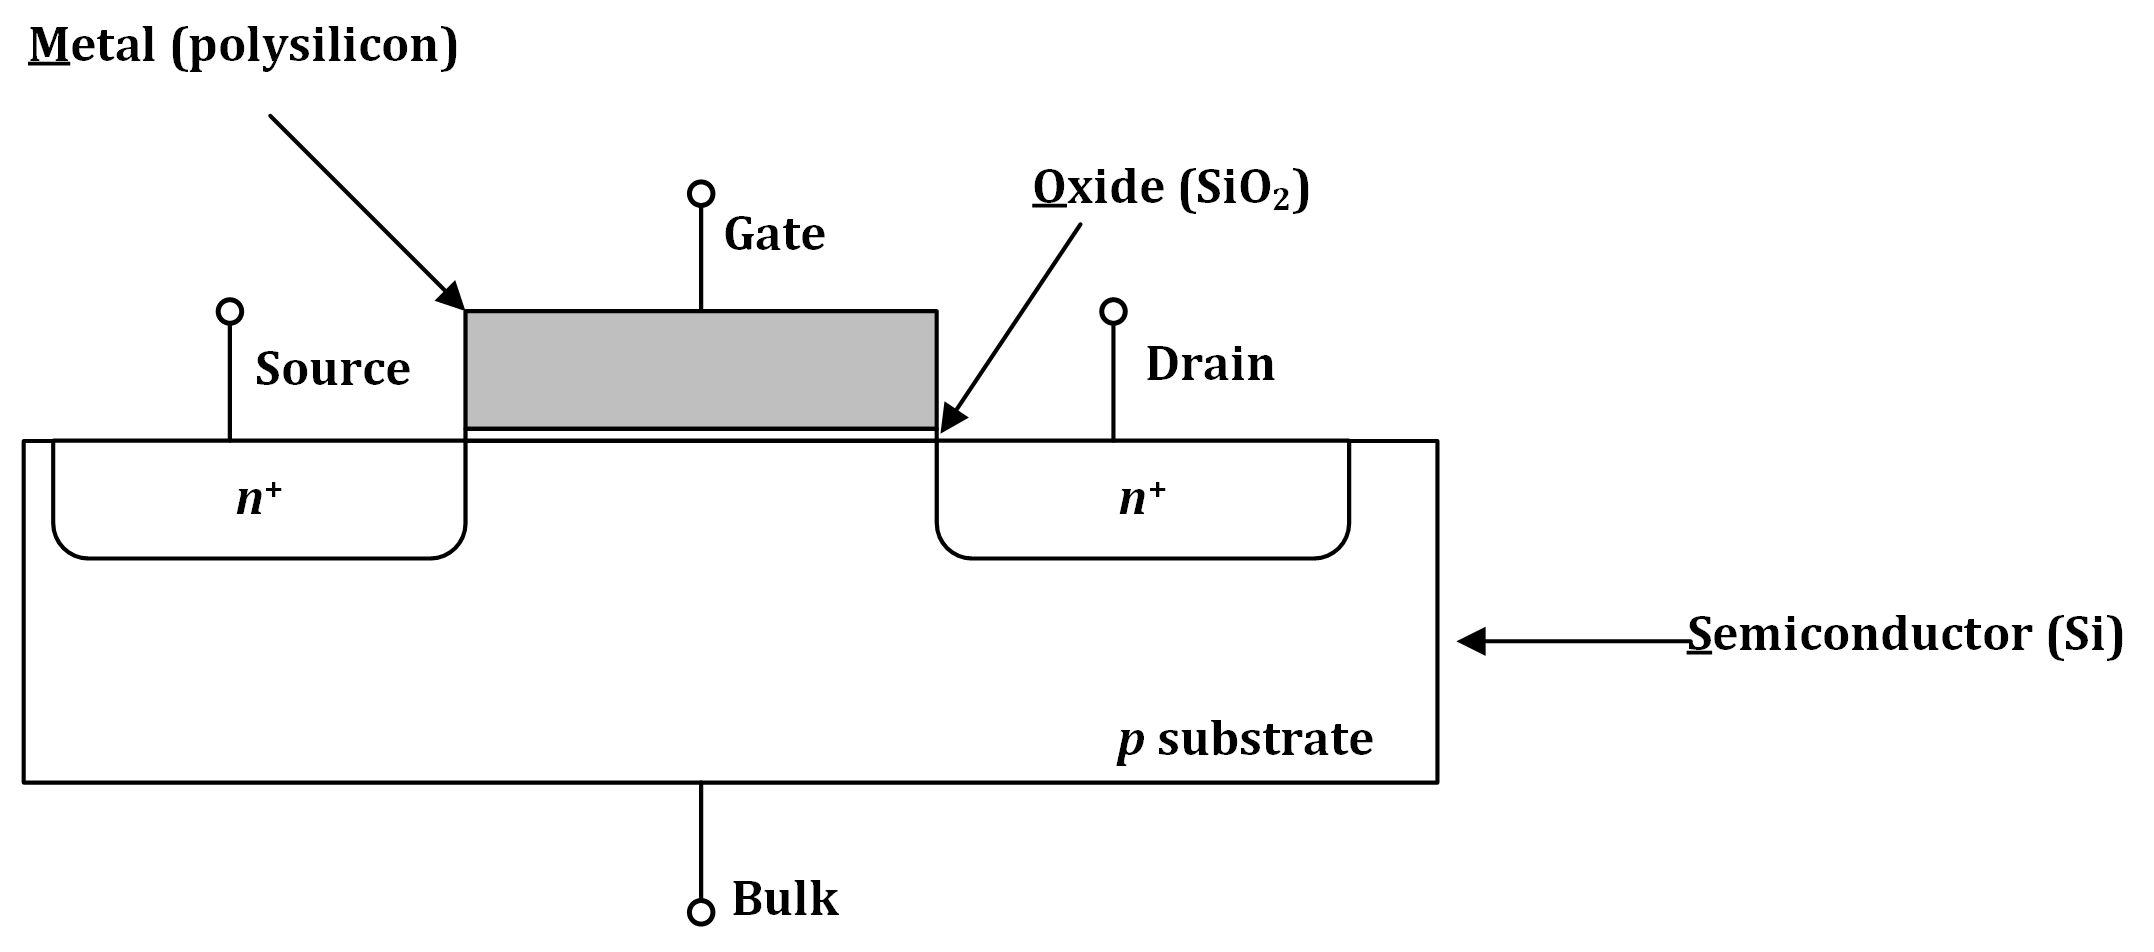
\includegraphics{MOS_structure.png}
\caption{MOS\_structure.png}
\end{figure}

    \begin{itemize}
\tightlist
\item
  MOSFET: \_\_M\_\_etal-\_\_O\_\_xide-\_\_S\_\_emiconductor
  \_\_F\_\_ield \_\_E\_\_ffect \_\_T\_\_ransistor
\item
  CMOS: \_\_C\_\_omplementary \textbf{MOS} (NMOS and PMOS in a single
  process)
\item
  n-type transistors (NMOS) consist of p-doped bulk, n-doped
  source/drain, polysilicon gate, and SiO2 insulating layer
\item
  p-type transistors (PMOS) have n-doped bulk, p-doped source/drain
\end{itemize}

    \hypertarget{nmos-operation}{%
\subsection{NMOS operation}\label{nmos-operation}}

    \begin{figure}
\centering
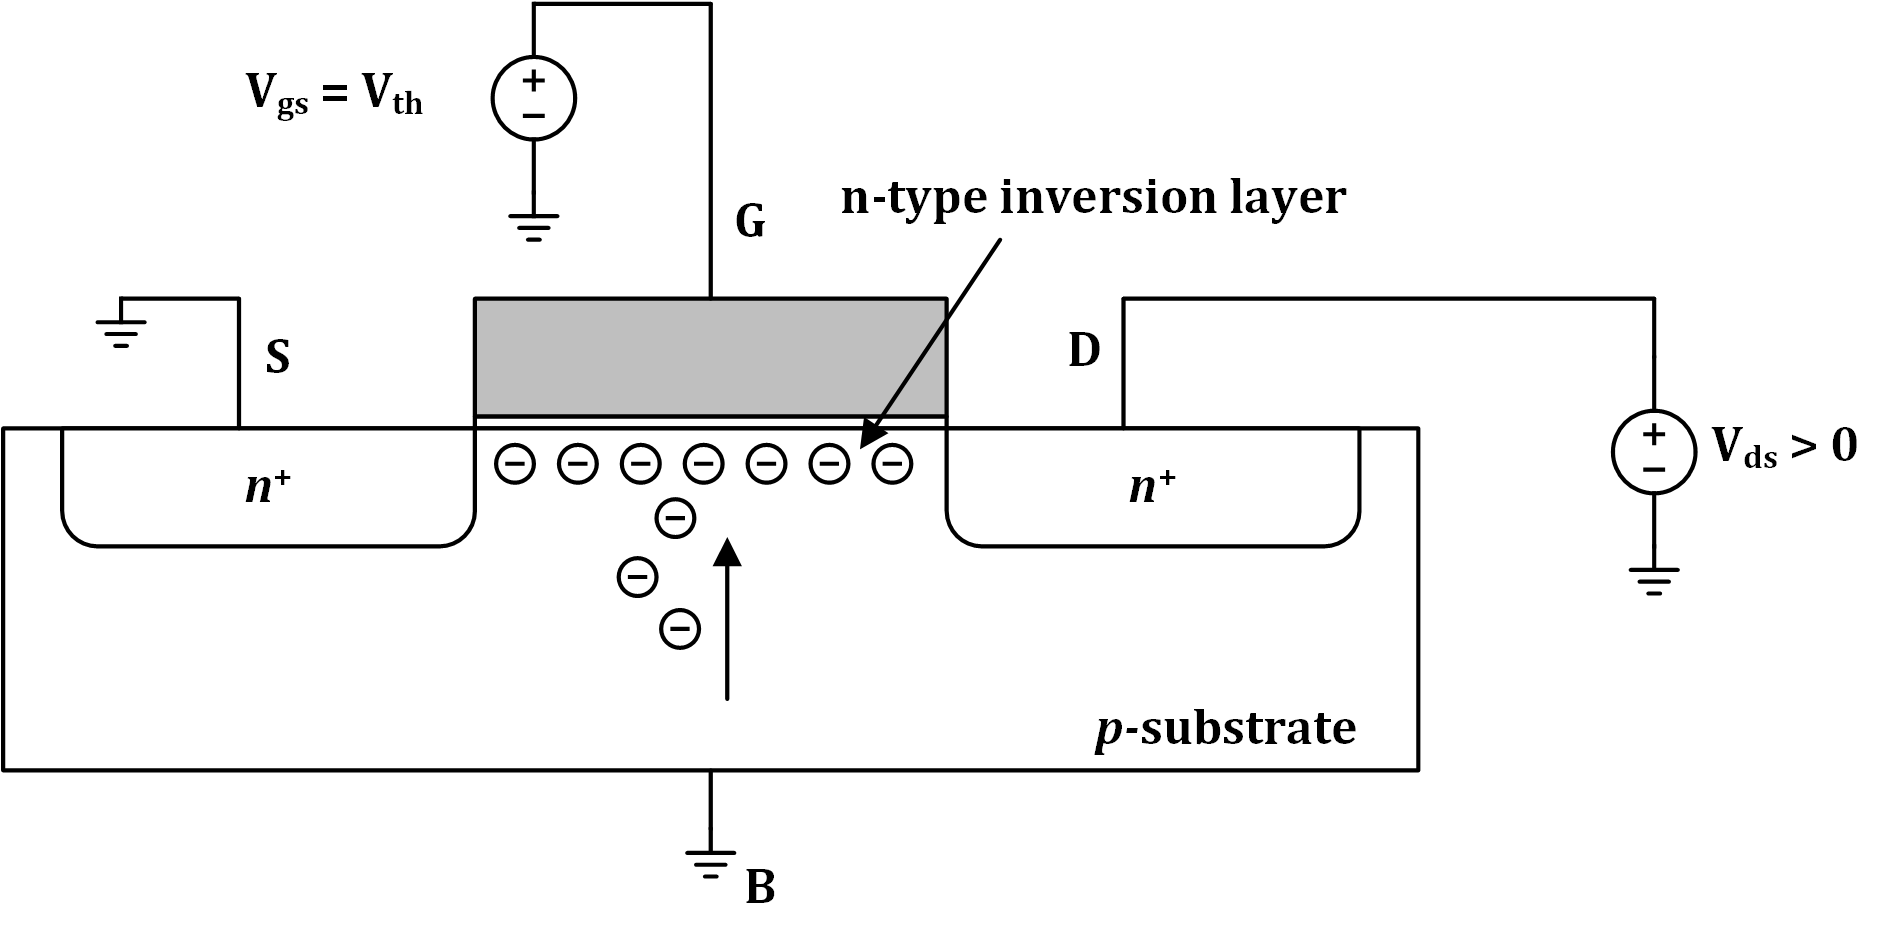
\includegraphics{NMOS_operation.png}
\caption{NMOS\_operation.png}
\end{figure}

    \begin{itemize}
\tightlist
\item
  In the absence of an applied gate-source voltage (\(V_{gs}\)), the
  charge concentration under the gate is dominated by \emph{majority}
  carriers (holes for an NMOS)
\item
  An \emph{inversion layer} begins to form as minority carriers are
  drawn from bulk to interface for \(V_{gs} > 0\)
\item
  Threshold voltage (\(V_{th}\)) is defined as the \(V_{gs}\) value at
  which the minority carrier (electron) concentration equals that of the
  majority carriers (holes)
\end{itemize}

    \hypertarget{nmos-operation}{%
\subsection{NMOS operation}\label{nmos-operation}}

    \begin{figure}
\centering
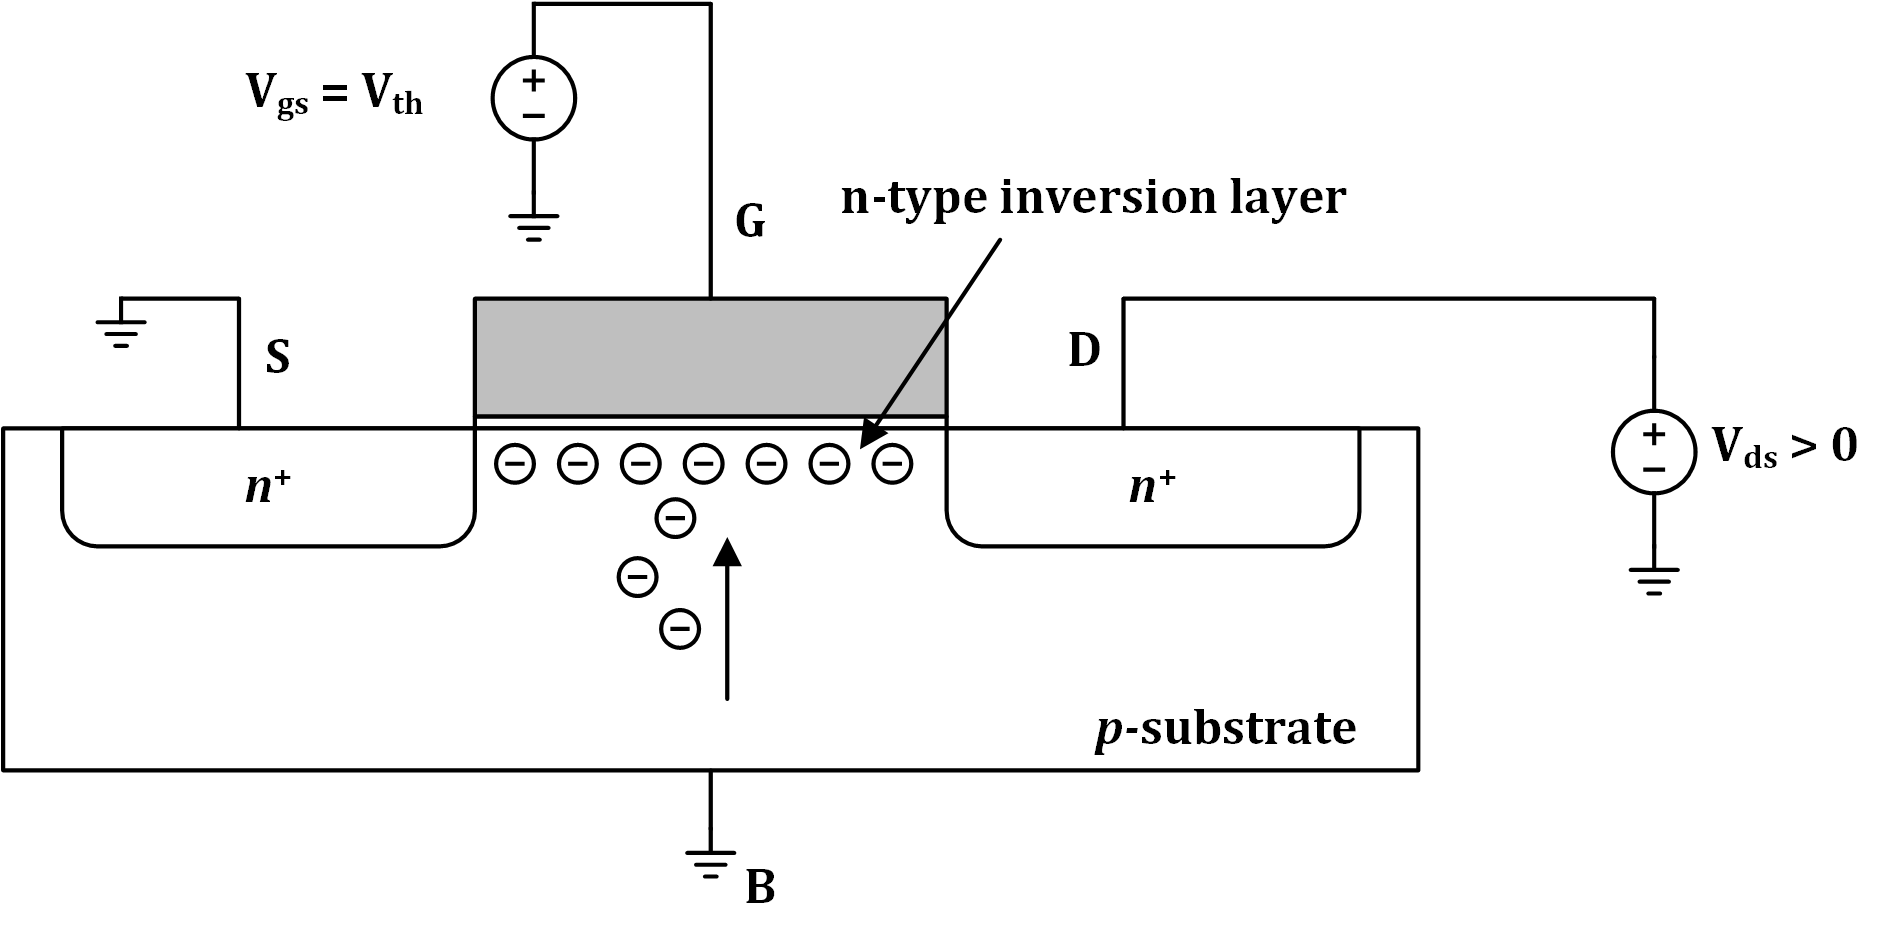
\includegraphics{NMOS_operation.png}
\caption{NMOS\_operation.png}
\end{figure}

    \begin{itemize}
\tightlist
\item
  Current is controlled by the velocity of mobile charge in the channel
\item
  Vertical electric field (\(E_{vert}\)) controls charge density
\item
  Carrier velocity proportional to lateral electric field
  (\(v=\mu E_{lat}\))
\item
  Our goal: Calculate drain current as a function of \(V_{gs}\) and
  \(V_{ds}\)
\end{itemize}

    \hypertarget{vertical-electric-field}{%
\subsection{Vertical electric field}\label{vertical-electric-field}}

    \begin{figure}
\centering
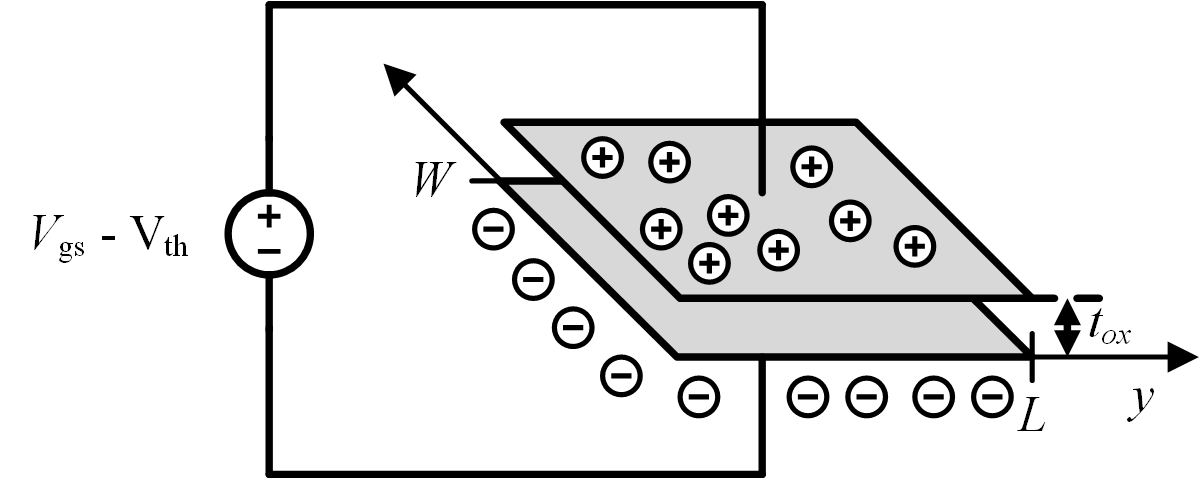
\includegraphics{MOS_vertical_field.png}
\caption{MOS\_vertical\_field.png}
\end{figure}

    \begin{itemize}
\tightlist
\item
  \(C_{ox}\): Oxide capacitance, in \(F/m^2\)
\item
  Charge per unit area, \(Q(y)\), depends on \(V_{gs} - V_{th}\),
  \(\epsilon_{ox}\), and \(t_{ox}\):
\end{itemize}

\begin{equation}
Q(y) = C_{ox}[V_{gs} - V_{th} - V(y)] = \dfrac{\epsilon_{ox}}{t_{ox}}[V_{gs} - V_{th} - V(y)]
\end{equation} - Vertical electric field controls channel charge density

    \hypertarget{lateral-electric-field}{%
\subsection{Lateral electric field}\label{lateral-electric-field}}

    \begin{figure}
\centering
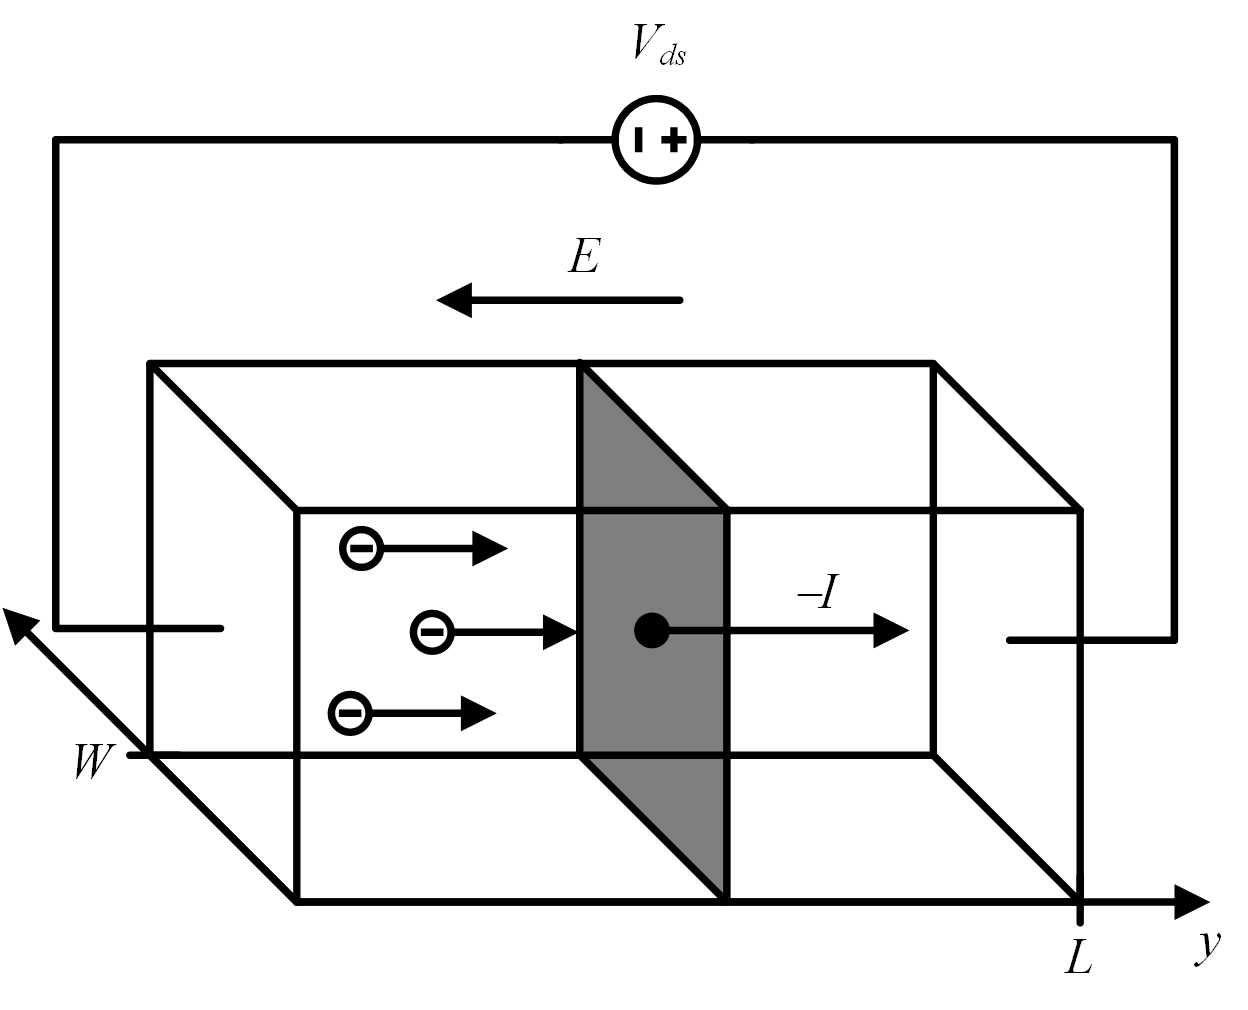
\includegraphics{MOS_lateral_field.png}
\caption{MOS\_lateral\_field.png}
\end{figure}

    \begin{itemize}
\tightlist
\item
  Current is controlled by charge density, mobility, and applied
  voltage:
\end{itemize}

\begin{align}
I &= Q(y) \cdot v\\
&= Q(y) \cdot \mu \cdot E_{lat} \\
&= Q(y) \cdot \mu \cdot \dfrac{dV(y)}{dy}
\end{align}

\begin{itemize}
\tightlist
\item
  While the vertical electric field controls charge density, the lateral
  electric field controls charge velocity
\end{itemize}

    \hypertarget{first-order-i-v-characteristics}{%
\subsection{First-order I-V
characteristics}\label{first-order-i-v-characteristics}}

    \begin{figure}
\centering
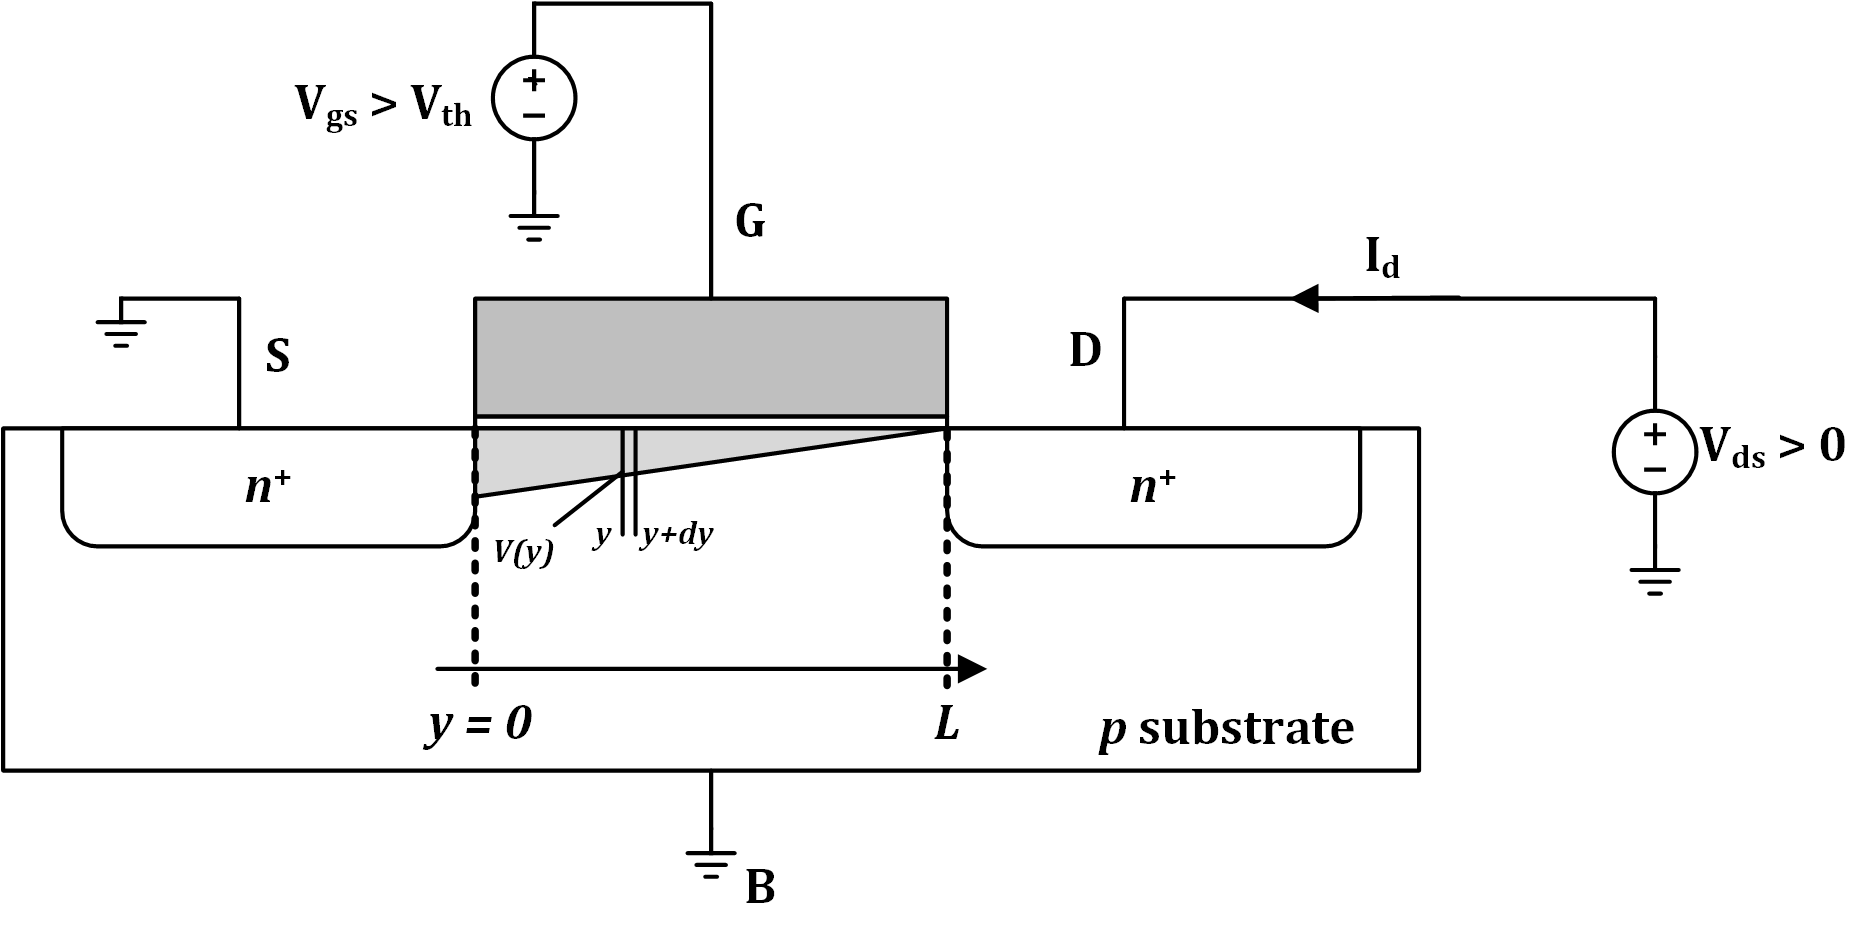
\includegraphics{MOS_IV_cross_section.png}
\caption{MOS\_IV\_cross\_section.png}
\end{figure}

    \begin{itemize}
\tightlist
\item
  Charge density and velocity:
\end{itemize}

\begin{equation}
Q_n(y) = C_{ox}[V_{gs} - V_{th} - V(y)]
\end{equation}

\begin{equation}
v = \mu \cdot E_{lat}
\end{equation}

    \begin{itemize}
\tightlist
\item
  Resulting drain current:
\end{itemize}

\begin{align}
I_d &= Q_n \cdot v \cdot W \\
\\
&= C_{ox}[V_{gs} - V_{th} - V(y)] \cdot \mu \cdot E_{lat} \cdot W \\
\end{align}

    \hypertarget{mos-i-v-derivation}{%
\subsection{MOS I-V derivation}\label{mos-i-v-derivation}}

    \begin{align}
I_d &= C_{ox}[V_{gs} - V_{th} - V(y)] \cdot \mu \cdot E \cdot W \\
\\
I_d \cdot dy &= \mu \cdot C_{ox} \cdot W [V_{gs} - V_{th} - V(y)]\cdot dV \\
\\
I_d \int_0^L{dy} &= \mu \cdot C_{ox} \cdot W  \int_0^{V_{ds}}{[V_{gs} - V_{th} - V(y)]\cdot dV}\\
\end{align}

\[\boxed{I_d = \mu \cdot C_{ox} \cdot \dfrac{W}{L} {\left[(V_{gs} - V_{th}) - \dfrac{V_{ds}}{2}\right]\cdot V_{ds}}} \]

\begin{itemize}
\tightlist
\item
  Drain current is the product of chrage density and velocity
\item
  Due to the variation in potential from source to drain, charge density
  must be integrated to determine the drain current
\item
  Let's plot the resulting function\ldots{}
\end{itemize}

    \hypertarget{first-order-i-v-characteristic}{%
\subsection{First-order I-V
characteristic}\label{first-order-i-v-characteristic}}

    \begin{tcolorbox}[breakable, size=fbox, boxrule=1pt, pad at break*=1mm,colback=cellbackground, colframe=cellborder]
\prompt{In}{incolor}{3}{\boxspacing}
\begin{Verbatim}[commandchars=\\\{\}]
\PY{n}{u\PYZus{}n} \PY{o}{=} \PY{l+m+mi}{350}                 \PY{c+c1}{\PYZsh{} electron mobility (device parameter)}
\PY{n}{e\PYZus{}ox} \PY{o}{=} \PY{l+m+mf}{3.9}\PY{o}{*}\PY{l+m+mf}{8.854e\PYZhy{}12}\PY{o}{/}\PY{l+m+mi}{100}\PY{p}{;} \PY{c+c1}{\PYZsh{} relative permittivity}
\PY{n}{t\PYZus{}ox} \PY{o}{=} \PY{l+m+mf}{9e\PYZhy{}9}\PY{o}{*}\PY{l+m+mi}{100}\PY{p}{;}          \PY{c+c1}{\PYZsh{} oxide thickness}
\PY{n}{C\PYZus{}ox} \PY{o}{=} \PY{n}{e\PYZus{}ox}\PY{o}{/}\PY{n}{t\PYZus{}ox}          \PY{c+c1}{\PYZsh{} oxide capacitance}
\PY{n}{V\PYZus{}th} \PY{o}{=} \PY{l+m+mf}{0.7}                \PY{c+c1}{\PYZsh{} threshold voltage (device parameter)}
\PY{n}{W} \PY{o}{=} \PY{l+m+mi}{100}                   \PY{c+c1}{\PYZsh{} device width in microns}
\PY{n}{L} \PY{o}{=} \PY{l+m+mi}{1}                     \PY{c+c1}{\PYZsh{} device length in microns}

\PY{n}{V\PYZus{}ds} \PY{o}{=} \PY{n}{np}\PY{o}{.}\PY{n}{arange}\PY{p}{(}\PY{l+m+mi}{0}\PY{p}{,}\PY{l+m+mf}{2.65}\PY{p}{,}\PY{n}{step}\PY{o}{=}\PY{l+m+mf}{0.05}\PY{p}{)}
\PY{n}{V\PYZus{}gs} \PY{o}{=} \PY{l+m+mi}{2}
\PY{n}{I\PYZus{}d} \PY{o}{=} \PY{n}{u\PYZus{}n}\PY{o}{*}\PY{n}{C\PYZus{}ox}\PY{o}{*}\PY{p}{(}\PY{n}{W}\PY{o}{/}\PY{n}{L}\PY{p}{)}\PY{o}{*}\PY{p}{(}\PY{n}{V\PYZus{}gs} \PY{o}{\PYZhy{}} \PY{n}{V\PYZus{}th} \PY{o}{\PYZhy{}} \PY{n}{V\PYZus{}ds}\PY{o}{/}\PY{l+m+mi}{2}\PY{p}{)}\PY{o}{*}\PY{n}{V\PYZus{}ds} 
\end{Verbatim}
\end{tcolorbox}

    \begin{tcolorbox}[breakable, size=fbox, boxrule=1pt, pad at break*=1mm,colback=cellbackground, colframe=cellborder]
\prompt{In}{incolor}{4}{\boxspacing}
\begin{Verbatim}[commandchars=\\\{\}]
\PY{n}{plot\PYZus{}xy}\PY{p}{(}\PY{n}{V\PYZus{}ds}\PY{p}{,} \PY{n}{I\PYZus{}d}\PY{p}{,} \PY{l+s+sa}{r}\PY{l+s+s1}{\PYZsq{}}\PY{l+s+s1}{\PYZdl{}V\PYZus{}}\PY{l+s+si}{\PYZob{}ds\PYZcb{}}\PY{l+s+s1}{ [V]\PYZdl{}}\PY{l+s+s1}{\PYZsq{}}\PY{p}{,} \PY{l+s+s1}{\PYZsq{}}\PY{l+s+s1}{\PYZdl{}I\PYZus{}d [A]\PYZdl{}}\PY{l+s+s1}{\PYZsq{}}\PY{p}{)}
\end{Verbatim}
\end{tcolorbox}

    \begin{center}
    \adjustimage{max size={0.9\linewidth}{0.9\paperheight}}{output_45_0.png}
    \end{center}
    { \hspace*{\fill} \\}
    
    \begin{itemize}
\tightlist
\item
  \(I_d\) appears to be decreasing for \(V_{ds} > V_{gs} - V_{th}\)
\item
  What really happens when \(V_{ds} > V_{gs} - V_{th}\)?
\item
  When the potential near the drain region is high enough such that
  \(V_{gd} = V_{gs} - V_{ds} < V_{th}\), the inversion charge becomes
  zero (a phenomenon known as ``pinch-off'')
\end{itemize}

    \hypertarget{first-order-i-v-characteristics-revisited}{%
\subsection{First-order I-V characteristics,
revisited}\label{first-order-i-v-characteristics-revisited}}

    \begin{figure}
\centering
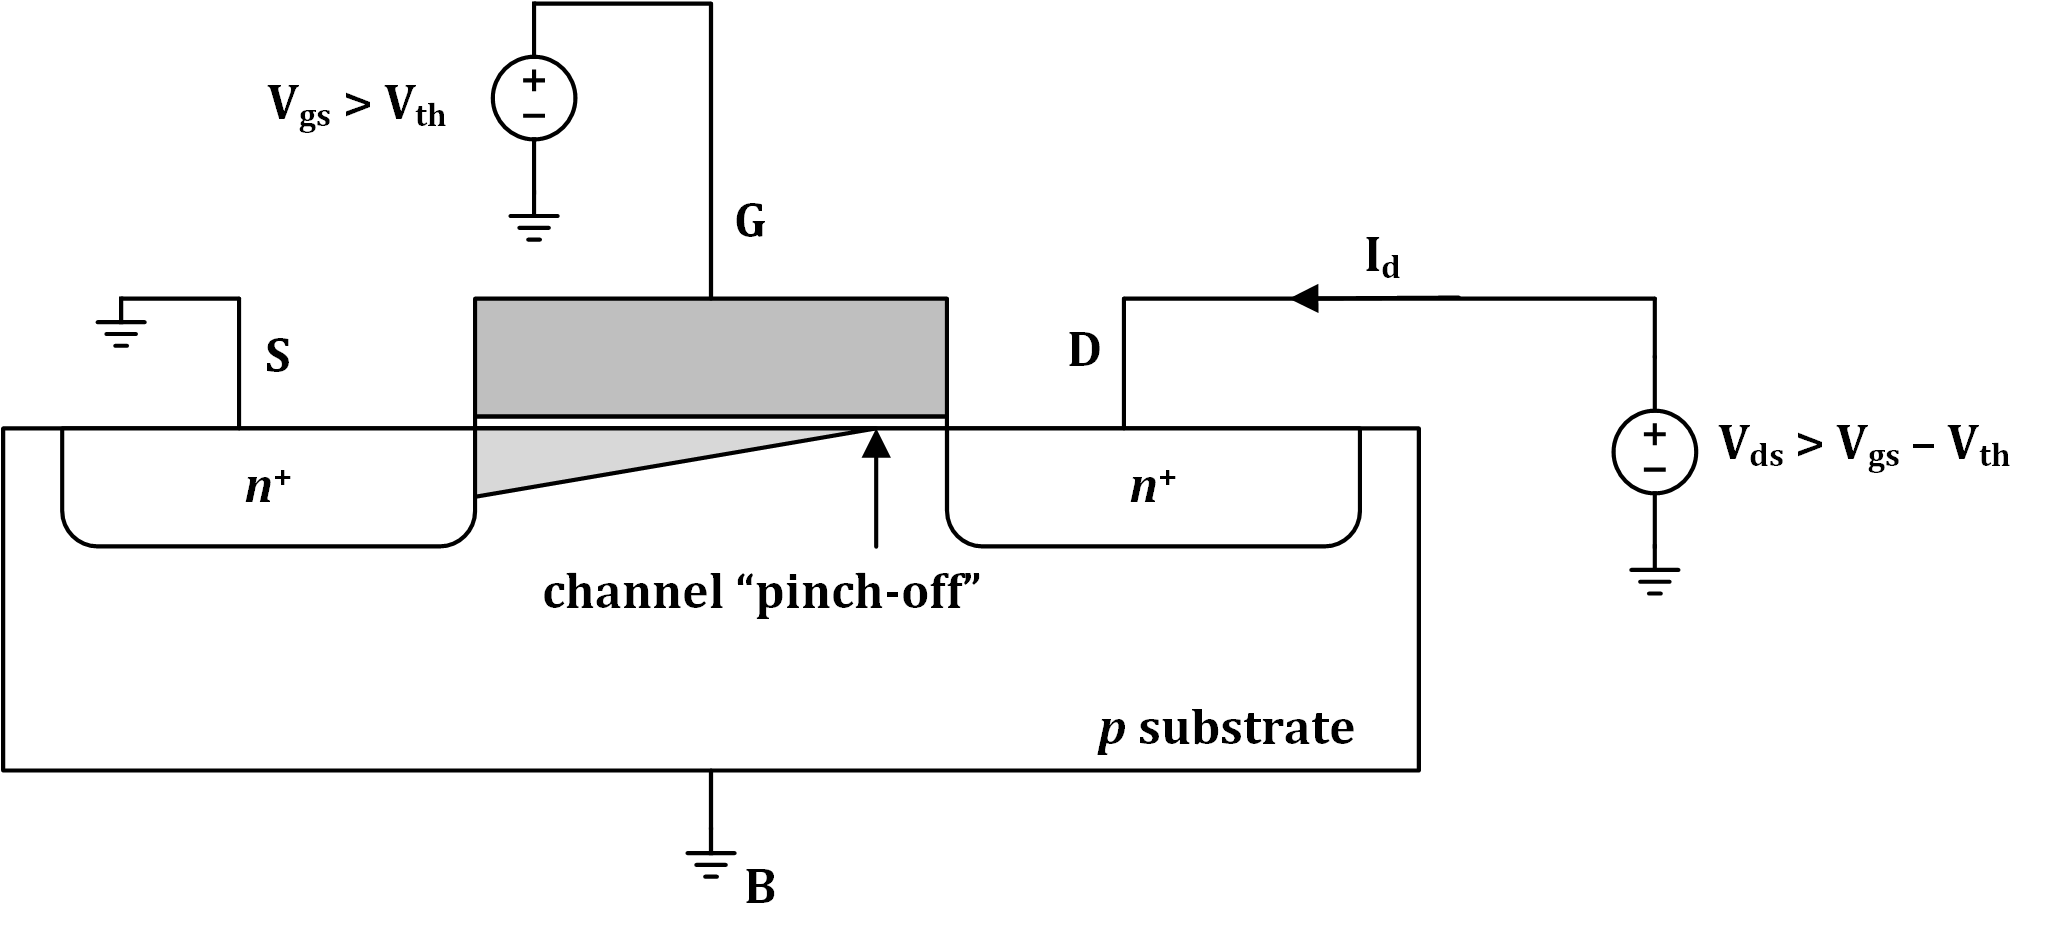
\includegraphics{NMOS_pinch_off.png}
\caption{NMOS\_pinch\_off.png}
\end{figure}

    \begin{itemize}
\tightlist
\item
  Near the drain region, charge density is dependent on \(V_{gd}\), not
  \(V_{gs}\)
\item
  The absence of inversion charge in this region results in high
  \(E\)-field region, across which the excess \(V_{ds}\) drops
\item
  For \(V_{ds} > V_{gs} - V_{th}\), drain current becomes ``saturated,''
  no longer increasing with \(V_{ds}\)
\end{itemize}

    \hypertarget{mos-saturation-operation}{%
\subsection{MOS saturation operation}\label{mos-saturation-operation}}

    \begin{figure}
\centering
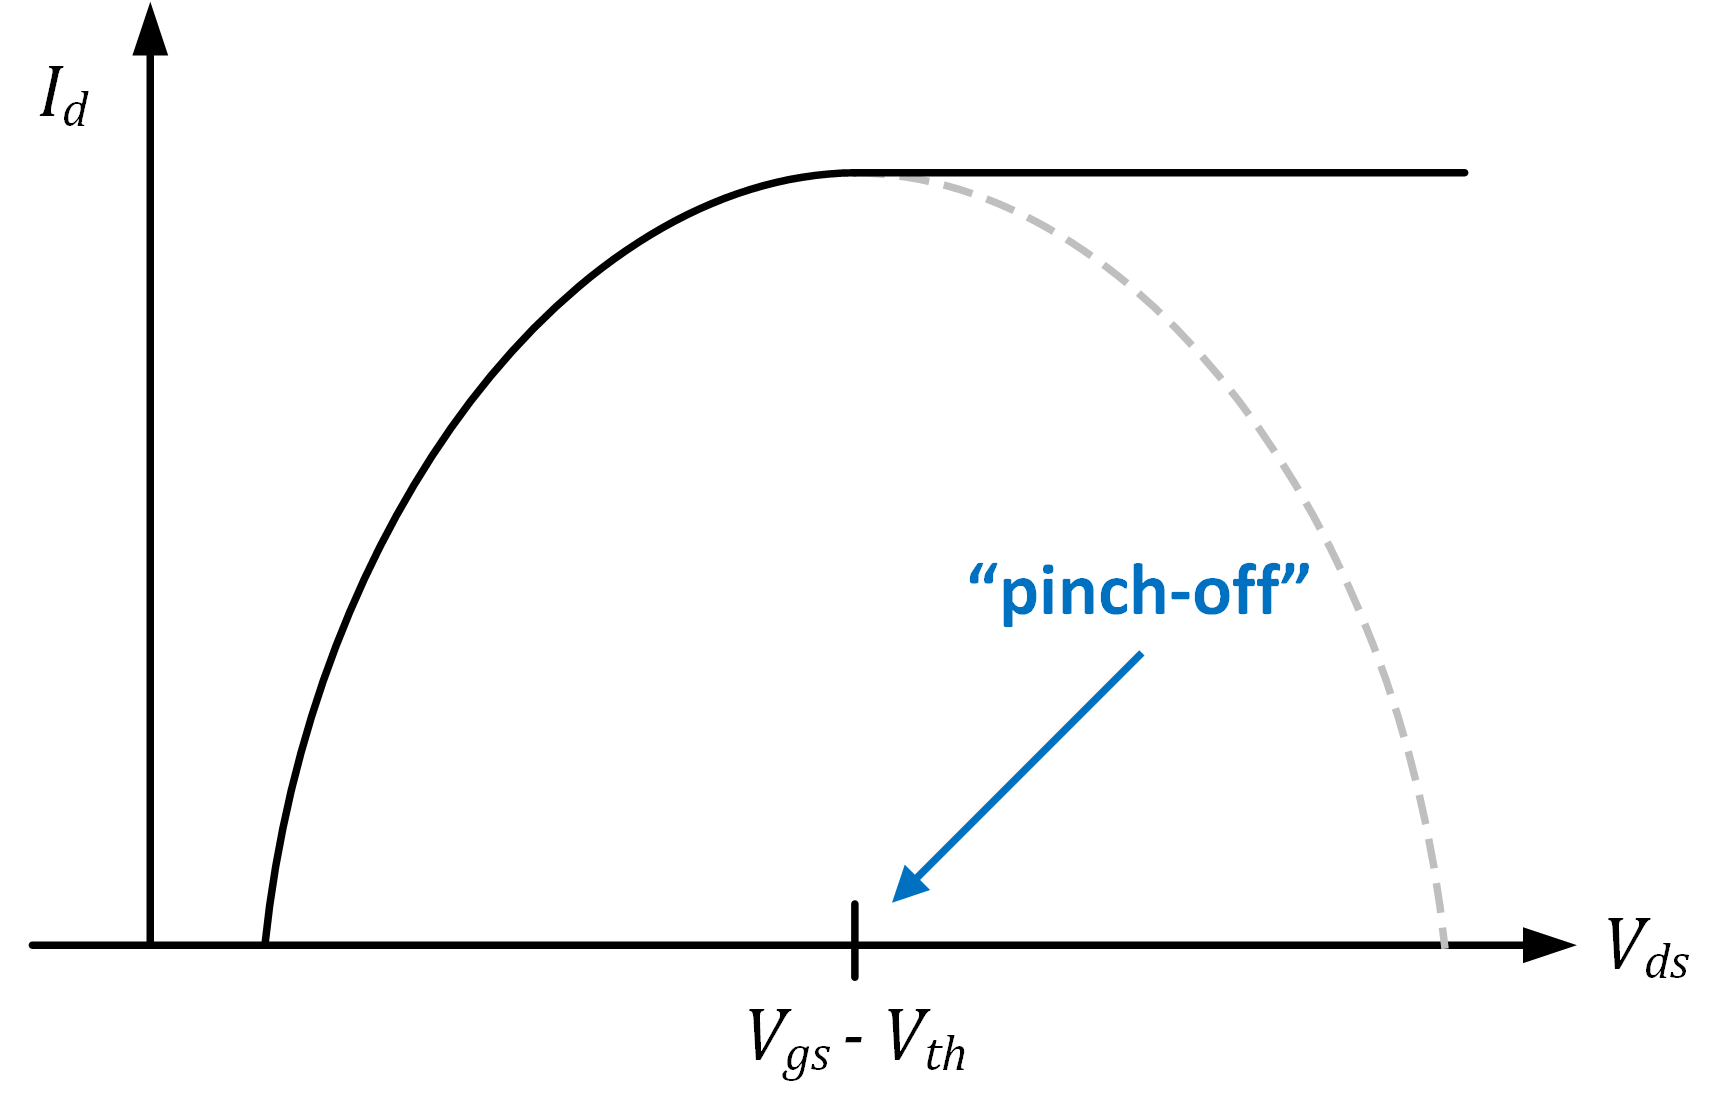
\includegraphics{MOS_saturation.png}
\caption{MOS\_saturation.png}
\end{figure}

    \begin{itemize}
\tightlist
\item
  In saturation, \(I_{d}\) is independent of \(V_{ds}\) (to first
  order), and is given by
\end{itemize}

\begin{equation}
I_d = \dfrac{1}{2}\mu\cdot C_{ox} \cdot \dfrac{W}{L}(V_{gs}-V_{th})^2
\end{equation}

\begin{itemize}
\tightlist
\item
  This behavior is what makes the MOS transistor effective as both a
  current source and a transconductance (gain) element
\item
  What about operation between \(V_{ds}=0\) and
  \(V_{ds}=V_{gs}-V_{th}\)?
\end{itemize}

    \hypertarget{mos-triode-operation}{%
\subsection{MOS triode operation}\label{mos-triode-operation}}

    \begin{align}
I_d &= \mu \cdot C_{ox} \cdot \dfrac{W}{L} {\left[(V_{gs} - V_{th}) - \dfrac{V_{ds}}{2}\right]\cdot V_{ds}}\\
\\
&= \mu \cdot C_{ox} \cdot \dfrac{W}{L} {\left[(V_{gs} - V_{th})\cdot V_{ds} - \dfrac{V_{ds}^2}{2}\right]}
\end{align}

\begin{itemize}
\tightlist
\item
  For \(V_{ds}\) \textless\textless{} \(V_{gs}-V_{th}\):
\end{itemize}

\begin{equation}
I_d \approx \mu \cdot C_{ox} \cdot \dfrac{W}{L} {(V_{gs} - V_{th})\cdot V_{ds}}
\end{equation}

    \begin{itemize}
\tightlist
\item
  For small values of \(V_{ds}\), drain current is approximately a
  linear function of \(V_{ds}\)
\item
  The MOS transistor in triode can thus be approximated as a resistance:
\end{itemize}

\begin{equation}
\boxed{R_{on} = \dfrac{V_{ds}}{I_d} \approx \dfrac{1}{\mu C_{ox} \dfrac{W}{L} (V_{gs} - V_{th})}} 
\end{equation}

\begin{itemize}
\tightlist
\item
  Though rarely used as an explicitly resistance, the MOS transistor is
  modeled this way when operated as a switch
\end{itemize}

    \hypertarget{mos-regions-of-operation}{%
\subsection{MOS regions of operation}\label{mos-regions-of-operation}}

    \begin{figure}
\centering
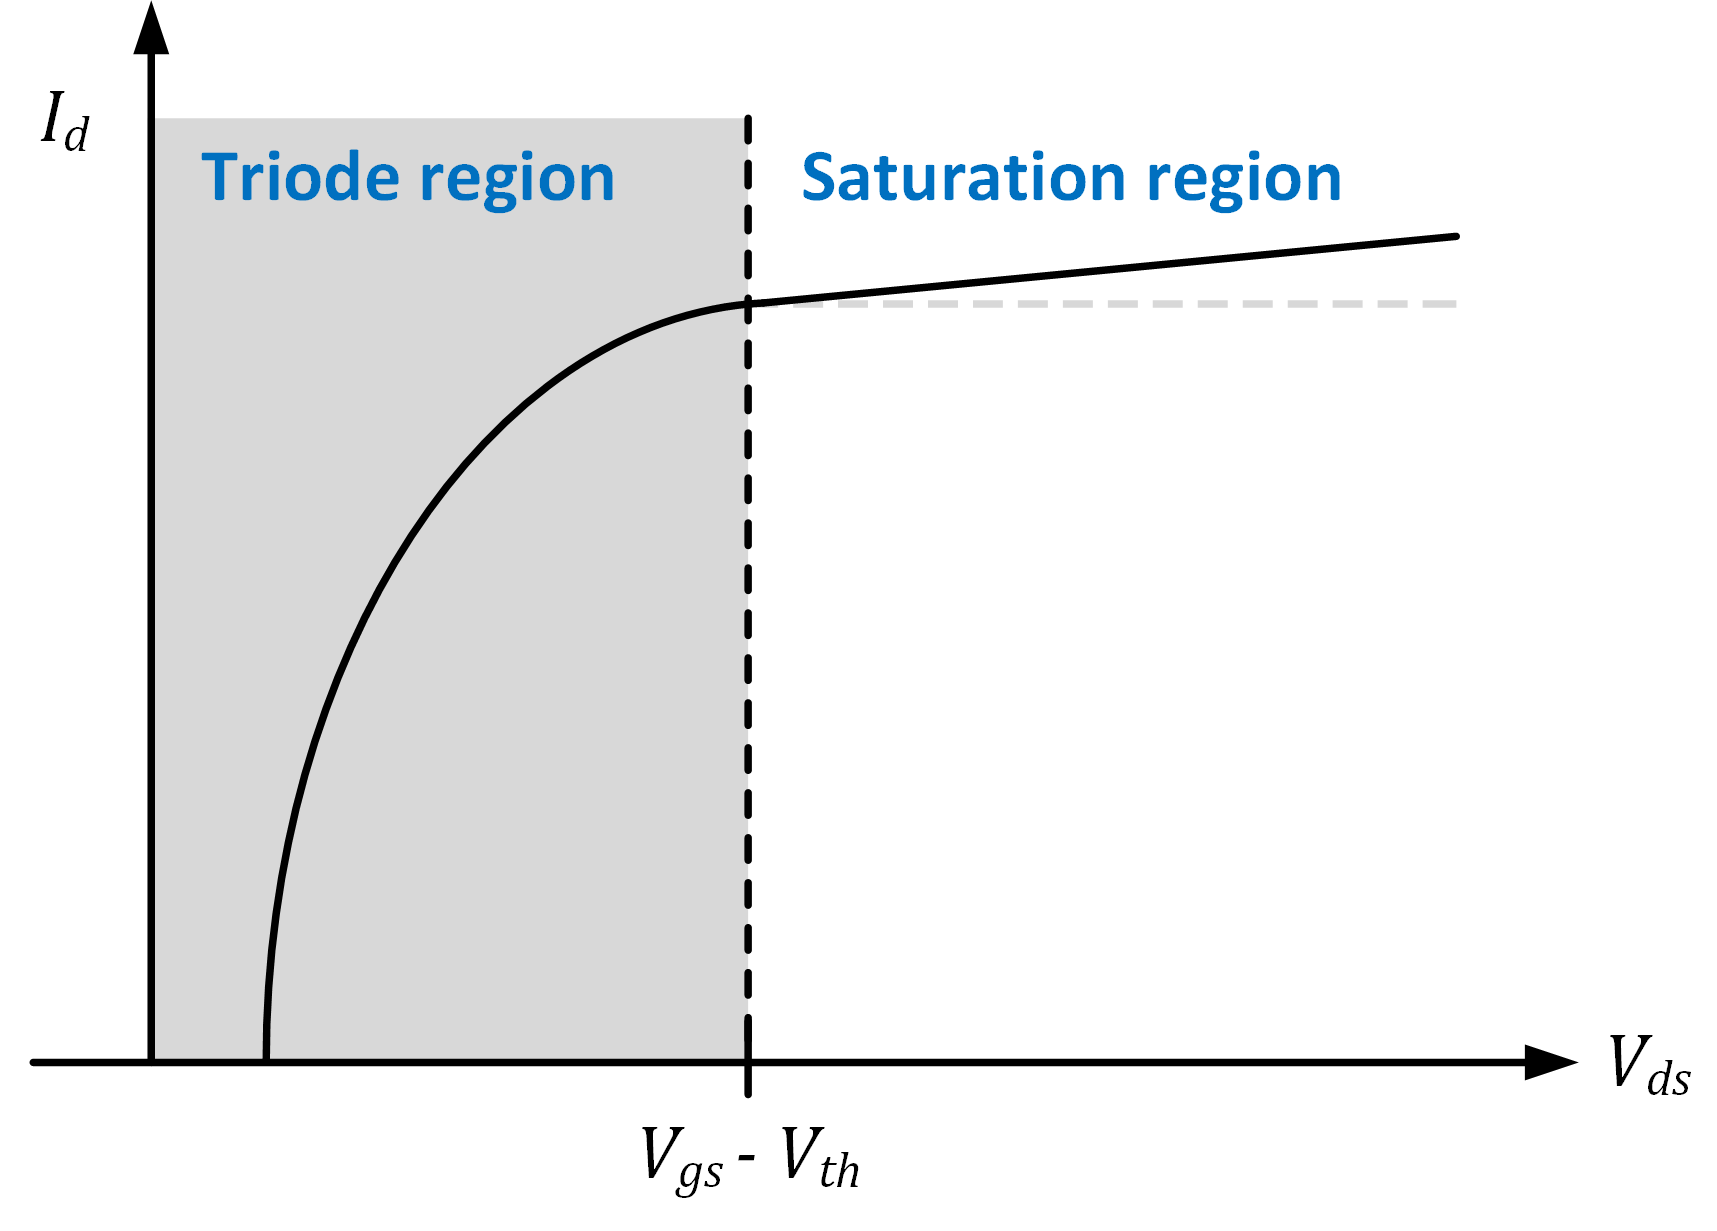
\includegraphics{MOS_regions.png}
\caption{MOS\_regions.png}
\end{figure}

    \begin{itemize}
\tightlist
\item
  Triode region expression:
\end{itemize}

\begin{equation}
I_d \approx \mu \cdot C_{ox} \cdot \dfrac{W}{L} {(V_{gs} - V_{th})\cdot V_{ds}}
\end{equation}

\begin{itemize}
\tightlist
\item
  Saturation region:
\end{itemize}

\begin{equation}
I_d \approx \dfrac{1}{2}\mu\cdot C_{ox} \cdot \dfrac{W}{L}(V_{gs}-V_{th})^2
\end{equation}

    \hypertarget{first-order-mos-model-summary}{%
\subsection{First-order MOS model
summary}\label{first-order-mos-model-summary}}

    \begin{figure}
\centering
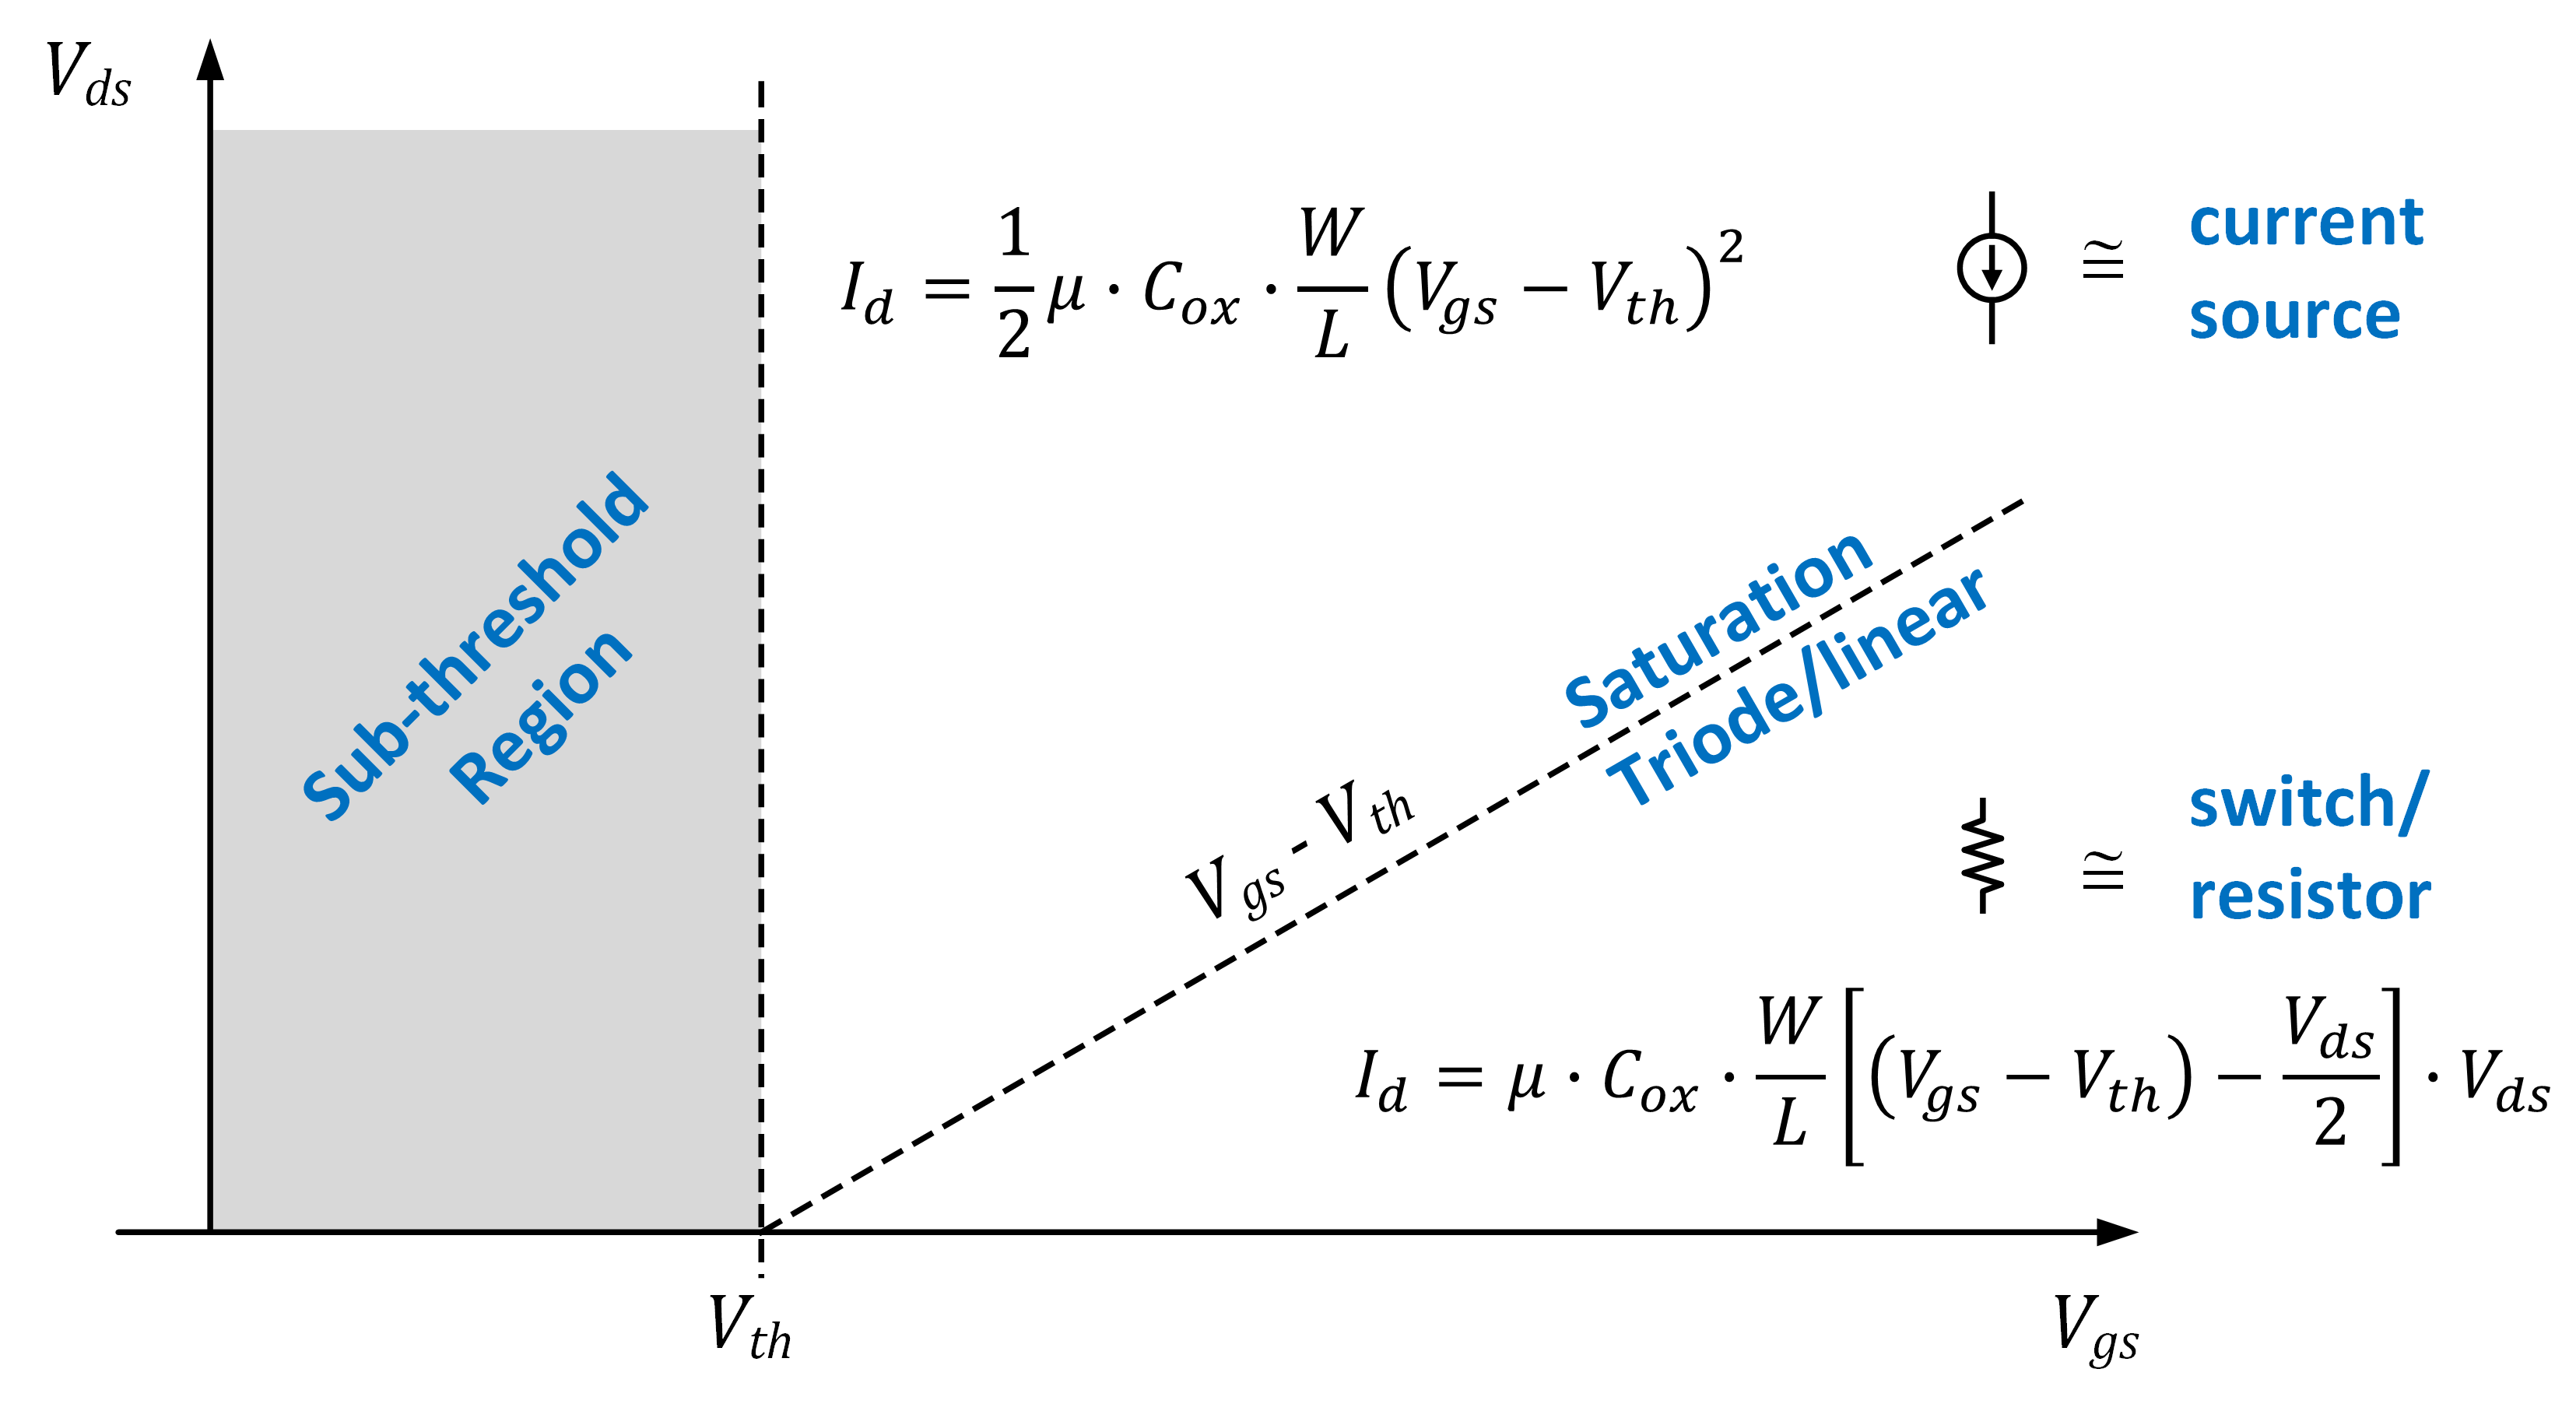
\includegraphics{MOS_regions_summary.png}
\caption{MOS\_regions\_summary.png}
\end{figure}

    \hypertarget{mos-i-v-characteristic}{%
\subsection{MOS I-V characteristic}\label{mos-i-v-characteristic}}

    \begin{tcolorbox}[breakable, size=fbox, boxrule=1pt, pad at break*=1mm,colback=cellbackground, colframe=cellborder]
\prompt{In}{incolor}{69}{\boxspacing}
\begin{Verbatim}[commandchars=\\\{\}]
\PY{k}{def} \PY{n+nf}{nmos\PYZus{}iv\PYZus{}sweep}\PY{p}{(}\PY{n}{V\PYZus{}gs}\PY{p}{,} \PY{n}{V\PYZus{}ds}\PY{p}{,} \PY{n}{W}\PY{p}{,} \PY{n}{L}\PY{p}{,} \PY{n}{lmda}\PY{p}{)}\PY{p}{:}
    \PY{n}{u\PYZus{}n} \PY{o}{=} \PY{l+m+mi}{350}                 \PY{c+c1}{\PYZsh{} electron mobility (device parameter)}
    \PY{n}{e\PYZus{}ox} \PY{o}{=} \PY{l+m+mf}{3.9}\PY{o}{*}\PY{l+m+mf}{8.854e\PYZhy{}12}\PY{o}{/}\PY{l+m+mi}{100}\PY{p}{;} \PY{c+c1}{\PYZsh{} relative permittivity}
    \PY{n}{t\PYZus{}ox} \PY{o}{=} \PY{l+m+mf}{9e\PYZhy{}9}\PY{o}{*}\PY{l+m+mi}{100}\PY{p}{;}          \PY{c+c1}{\PYZsh{} oxide thickness}
    \PY{n}{C\PYZus{}ox} \PY{o}{=} \PY{n}{e\PYZus{}ox}\PY{o}{/}\PY{n}{t\PYZus{}ox}          \PY{c+c1}{\PYZsh{} oxide capacitance}
    \PY{n}{V\PYZus{}th} \PY{o}{=} \PY{l+m+mf}{0.7}                \PY{c+c1}{\PYZsh{} threshold voltage (device parameter)}
    \PY{n}{V\PYZus{}ov} \PY{o}{=} \PY{n}{V\PYZus{}gs} \PY{o}{\PYZhy{}} \PY{n}{V\PYZus{}th}
    
    \PY{n}{I\PYZus{}d} \PY{o}{=} \PY{p}{[}\PY{p}{]}
    
    \PY{k}{for} \PY{n}{i} \PY{o+ow}{in} \PY{n+nb}{range}\PY{p}{(}\PY{n+nb}{len}\PY{p}{(}\PY{n}{V\PYZus{}ds}\PY{p}{)}\PY{p}{)}\PY{p}{:}
        \PY{n}{I\PYZus{}d}\PY{o}{.}\PY{n}{append}\PY{p}{(}\PY{n}{np}\PY{o}{.}\PY{n}{piecewise}\PY{p}{(}\PY{n}{V\PYZus{}ds}\PY{p}{[}\PY{n}{i}\PY{p}{]}\PY{p}{,} \PY{p}{[}\PY{n}{V\PYZus{}ds}\PY{p}{[}\PY{n}{i}\PY{p}{]} \PY{o}{\PYZlt{}} \PY{n}{V\PYZus{}ov}\PY{p}{,} \PY{n}{V\PYZus{}ds}\PY{p}{[}\PY{n}{i}\PY{p}{]} \PY{o}{\PYZgt{}}\PY{o}{=} \PY{n}{V\PYZus{}ov}\PY{p}{]}\PY{p}{,}
                       \PY{p}{[}\PY{n}{u\PYZus{}n}\PY{o}{*}\PY{n}{C\PYZus{}ox}\PY{o}{*}\PY{p}{(}\PY{n}{W}\PY{o}{/}\PY{n}{L}\PY{p}{)}\PY{o}{*}\PY{p}{(}\PY{n}{V\PYZus{}gs} \PY{o}{\PYZhy{}} \PY{n}{V\PYZus{}th} \PY{o}{\PYZhy{}} \PY{n}{V\PYZus{}ds}\PY{p}{[}\PY{n}{i}\PY{p}{]}\PY{o}{/}\PY{l+m+mi}{2}\PY{p}{)}\PY{o}{*}\PY{n}{V\PYZus{}ds}\PY{p}{[}\PY{n}{i}\PY{p}{]}\PY{o}{*}\PY{p}{(}\PY{l+m+mi}{1}\PY{o}{+}\PY{n}{lmda}\PY{o}{*}\PY{n}{V\PYZus{}ds}\PY{p}{[}\PY{n}{i}\PY{p}{]}\PY{p}{)} \PY{p}{,} 
                        \PY{l+m+mf}{0.5}\PY{o}{*}\PY{n}{u\PYZus{}n}\PY{o}{*}\PY{n}{C\PYZus{}ox}\PY{o}{*}\PY{p}{(}\PY{n}{W}\PY{o}{/}\PY{n}{L}\PY{p}{)}\PY{o}{*}\PY{p}{(}\PY{n}{V\PYZus{}gs} \PY{o}{\PYZhy{}} \PY{n}{V\PYZus{}th}\PY{p}{)}\PY{o}{*}\PY{o}{*}\PY{l+m+mi}{2}\PY{o}{*}\PY{p}{(}\PY{l+m+mi}{1}\PY{o}{+}\PY{n}{lmda}\PY{o}{*}\PY{n}{V\PYZus{}ds}\PY{p}{[}\PY{n}{i}\PY{p}{]}\PY{p}{)}\PY{p}{]}\PY{p}{)}\PY{p}{)} 
    
    \PY{k}{return} \PY{n}{np}\PY{o}{.}\PY{n}{array}\PY{p}{(}\PY{n}{I\PYZus{}d}\PY{p}{)}

\PY{k}{def} \PY{n+nf}{plot\PYZus{}ID\PYZus{}curves}\PY{p}{(}\PY{n}{V\PYZus{}gs}\PY{p}{,} \PY{n}{V\PYZus{}ds}\PY{p}{,} \PY{n}{W}\PY{p}{,} \PY{n}{L}\PY{p}{,} \PY{n}{lmda}\PY{p}{)}\PY{p}{:}
    \PY{n}{fig}\PY{p}{,} \PY{n}{ax} \PY{o}{=} \PY{n}{plt}\PY{o}{.}\PY{n}{subplots}\PY{p}{(}\PY{n}{figsize}\PY{o}{=}\PY{p}{(}\PY{l+m+mf}{10.0}\PY{p}{,}\PY{l+m+mf}{7.5}\PY{p}{)}\PY{p}{)}
    \PY{k}{for} \PY{n}{vgs} \PY{o+ow}{in} \PY{n}{V\PYZus{}gs}\PY{p}{:}
        \PY{n}{I\PYZus{}d} \PY{o}{=} \PY{n}{nmos\PYZus{}iv\PYZus{}sweep}\PY{p}{(}\PY{n}{vgs}\PY{p}{,} \PY{n}{V\PYZus{}ds}\PY{p}{,} \PY{n}{W}\PY{p}{,} \PY{n}{L}\PY{p}{,} \PY{n}{lmda}\PY{o}{=}\PY{n}{lmda}\PY{p}{)}
        \PY{n}{ax}\PY{o}{.}\PY{n}{plot}\PY{p}{(}\PY{n}{V\PYZus{}ds}\PY{p}{,} \PY{n}{I\PYZus{}d}\PY{p}{,} \PY{n}{label}\PY{o}{=}\PY{l+s+s1}{\PYZsq{}}\PY{l+s+s1}{Vgs = }\PY{l+s+s1}{\PYZsq{}}\PY{o}{+} \PY{n+nb}{str}\PY{p}{(}\PY{n}{vgs}\PY{p}{)}\PY{p}{)}
        \PY{n}{ax}\PY{o}{.}\PY{n}{set\PYZus{}xlabel}\PY{p}{(}\PY{l+s+sa}{r}\PY{l+s+s1}{\PYZsq{}}\PY{l+s+s1}{\PYZdl{}V\PYZus{}}\PY{l+s+si}{\PYZob{}ds\PYZcb{}}\PY{l+s+s1}{ [V]\PYZdl{}}\PY{l+s+s1}{\PYZsq{}}\PY{p}{)}
        \PY{n}{ax}\PY{o}{.}\PY{n}{set\PYZus{}ylabel}\PY{p}{(}\PY{l+s+sa}{r}\PY{l+s+s1}{\PYZsq{}}\PY{l+s+s1}{\PYZdl{}I\PYZus{}}\PY{l+s+si}{\PYZob{}D\PYZcb{}}\PY{l+s+s1}{ [mA]\PYZdl{}}\PY{l+s+s1}{\PYZsq{}}\PY{p}{)}
    \PY{n}{ax}\PY{o}{.}\PY{n}{grid}\PY{p}{(}\PY{p}{)}
    \PY{n}{ax}\PY{o}{.}\PY{n}{legend}\PY{p}{(}\PY{p}{)}    
\end{Verbatim}
\end{tcolorbox}

    \begin{tcolorbox}[breakable, size=fbox, boxrule=1pt, pad at break*=1mm,colback=cellbackground, colframe=cellborder]
\prompt{In}{incolor}{70}{\boxspacing}
\begin{Verbatim}[commandchars=\\\{\}]
\PY{n}{V\PYZus{}gs} \PY{o}{=} \PY{n}{np}\PY{o}{.}\PY{n}{arange}\PY{p}{(}\PY{l+m+mi}{1}\PY{p}{,} \PY{l+m+mi}{3}\PY{p}{,} \PY{n}{step}\PY{o}{=}\PY{o}{.}\PY{l+m+mi}{25}\PY{p}{)}
\PY{n}{V\PYZus{}ds} \PY{o}{=} \PY{n}{np}\PY{o}{.}\PY{n}{arange}\PY{p}{(}\PY{l+m+mi}{0}\PY{p}{,} \PY{l+m+mi}{5}\PY{p}{,} \PY{n}{step}\PY{o}{=}\PY{l+m+mf}{0.01}\PY{p}{)}
\PY{n}{W} \PY{o}{=} \PY{l+m+mi}{100}
\PY{n}{L} \PY{o}{=} \PY{l+m+mi}{1}
\end{Verbatim}
\end{tcolorbox}

    \begin{tcolorbox}[breakable, size=fbox, boxrule=1pt, pad at break*=1mm,colback=cellbackground, colframe=cellborder]
\prompt{In}{incolor}{71}{\boxspacing}
\begin{Verbatim}[commandchars=\\\{\}]
\PY{n}{plot\PYZus{}ID\PYZus{}curves}\PY{p}{(}\PY{n}{V\PYZus{}gs}\PY{p}{,} \PY{n}{V\PYZus{}ds}\PY{p}{,} \PY{l+m+mi}{100}\PY{p}{,} \PY{l+m+mi}{1}\PY{p}{,} \PY{l+m+mi}{0}\PY{p}{)}
\end{Verbatim}
\end{tcolorbox}

    \begin{center}
    \adjustimage{max size={0.9\linewidth}{0.9\paperheight}}{output_64_0.png}
    \end{center}
    { \hspace*{\fill} \\}
    
    \hypertarget{common-source-amplifier-spice-simulation}{%
\subsection{Common-source amplifier (SPICE
simulation)}\label{common-source-amplifier-spice-simulation}}

    \begin{figure}
\centering
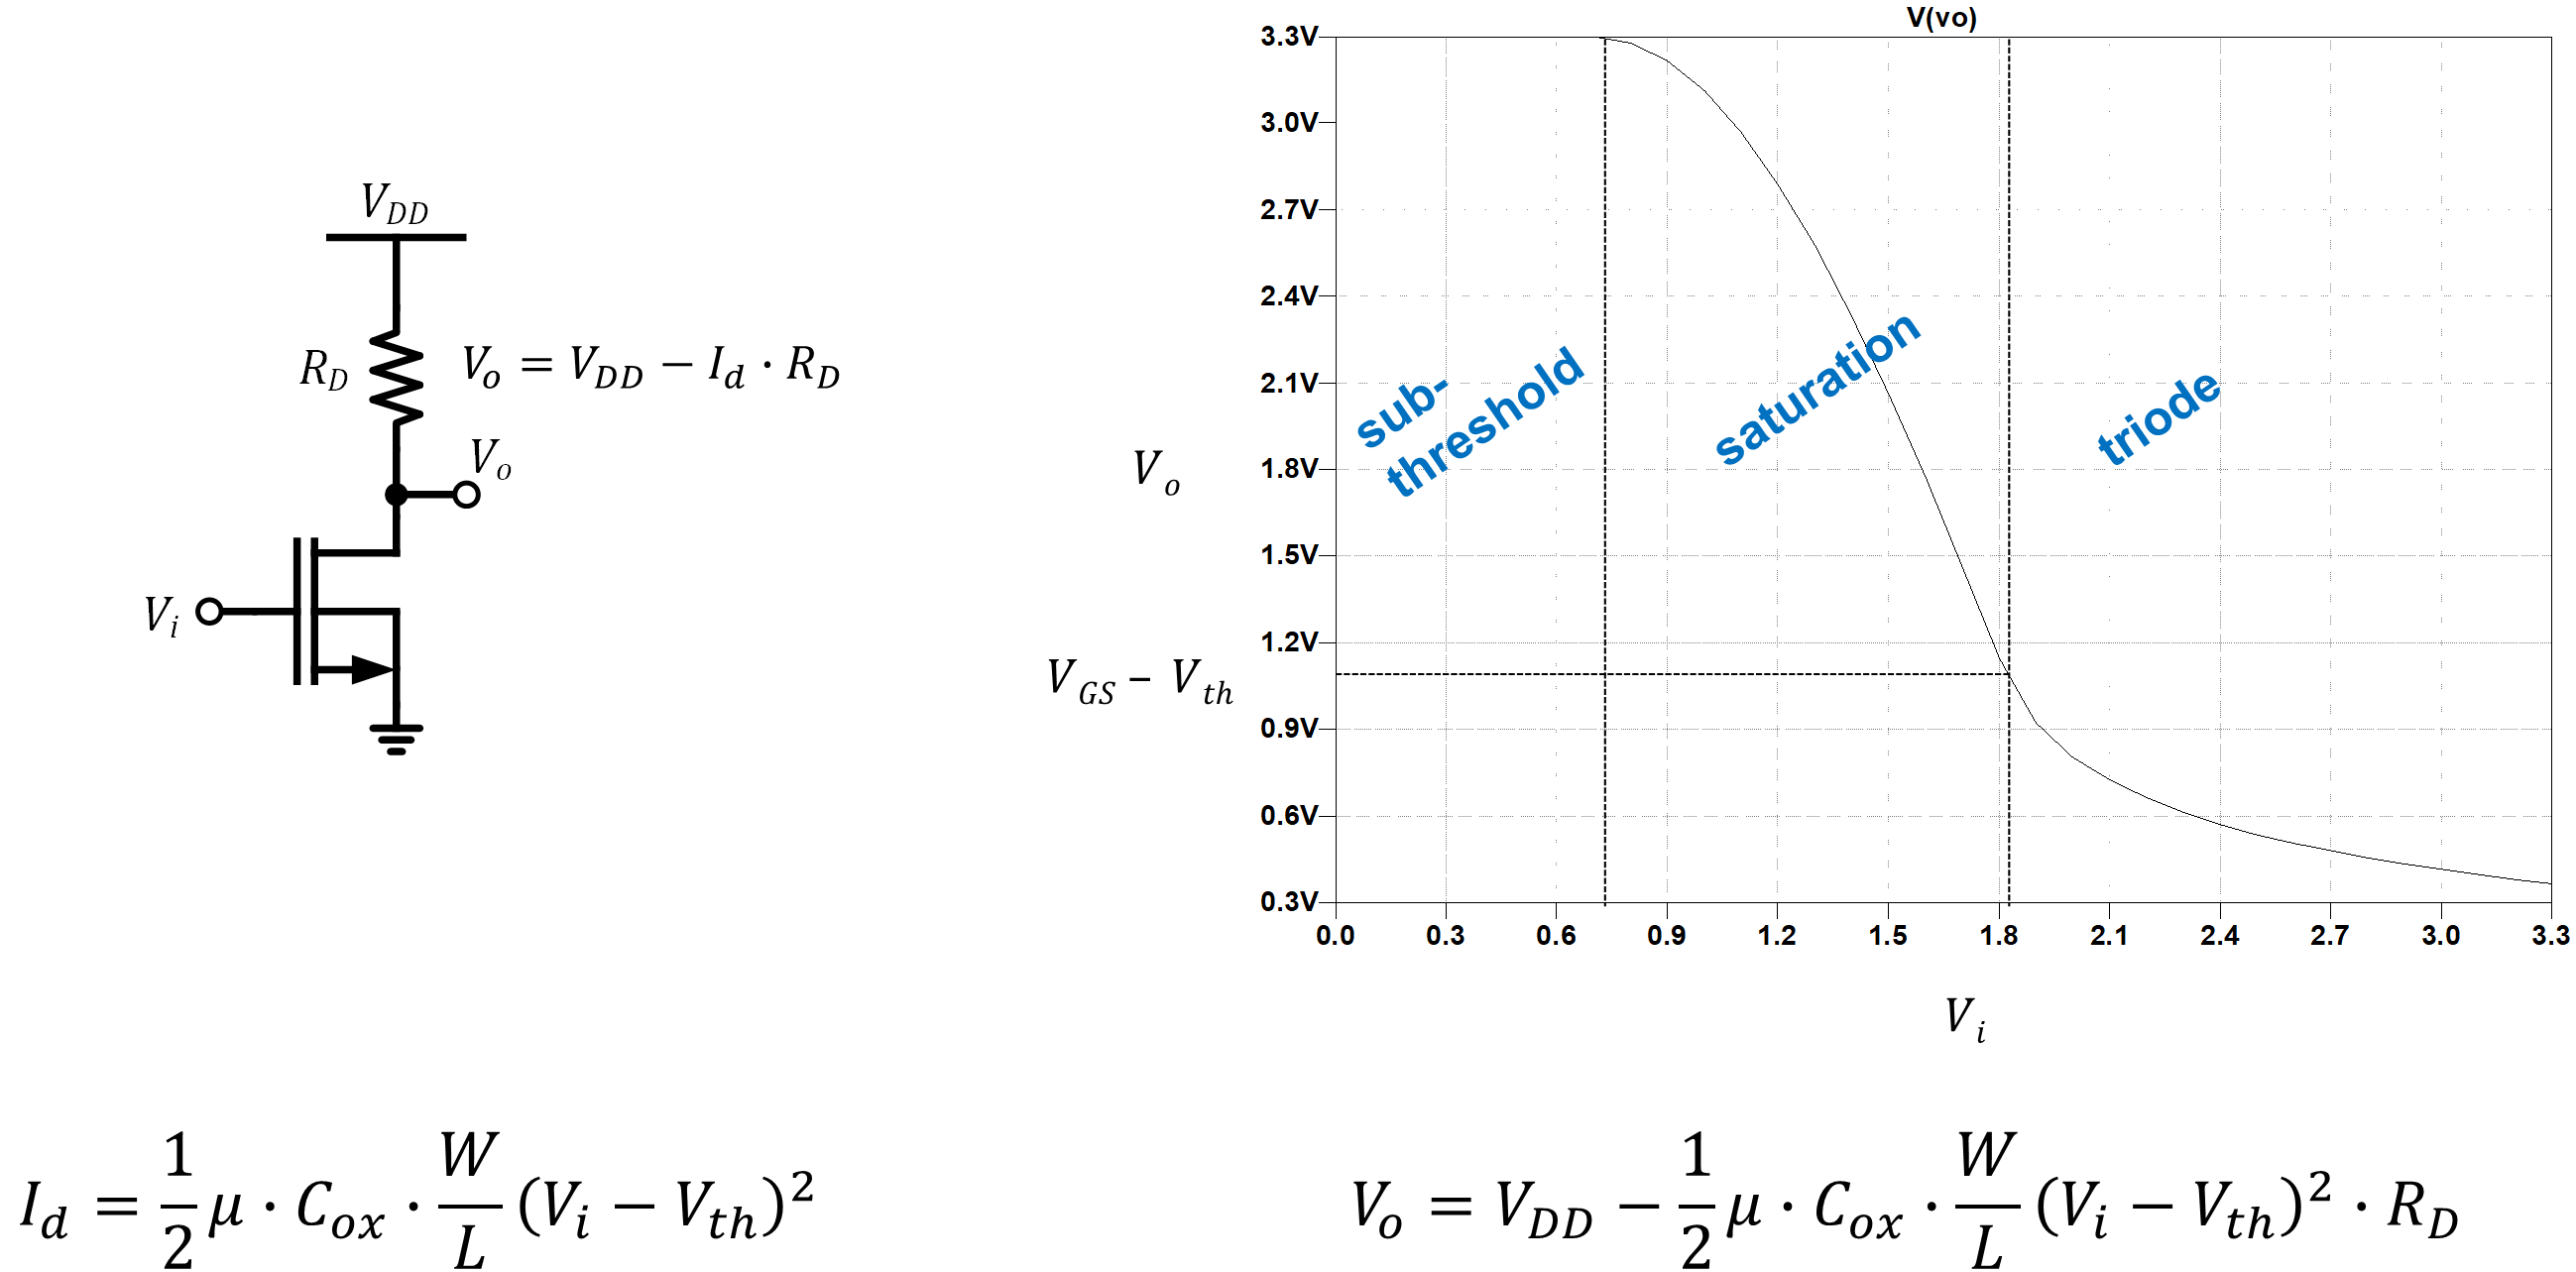
\includegraphics{common_source_sim.png}
\caption{common\_source\_sim.png}
\end{figure}

    \hypertarget{calculate-the-gain}{%
\subsection{Calculate the gain}\label{calculate-the-gain}}

    \begin{align}
V_o + \Delta V_o &= V_{DD} -  \dfrac{1}{2}\mu\cdot C_{ox} \cdot \dfrac{W}{L}(V_{gs} + \Delta V_i -V_{th})^2 \cdot R_D \\
\\
\Delta V_o &= -\dfrac{1}{2}\mu\cdot C_{ox} \cdot \dfrac{W}{L} \cdot R_D [(V_{ov} + \Delta V_i)^2 - V_{ov}^2 ] \\
\\
&= -\dfrac{1}{2}\mu\cdot C_{ox} \cdot \dfrac{W}{L} \cdot R_D [2V_{ov}\Delta V_i + \Delta V_i^2 ] \\
\\
&= -\dfrac{2I_d}{V_{ov}} \cdot R_D \Delta V_i \left[1+\dfrac{\Delta V_i}{2V_{ov}}\right ]
\end{align}

\begin{itemize}
\tightlist
\item
  The output voltage is quadratic in \(\Delta V_i\), but a linear
  approximation is sufficient for most purposes
\item
  Let's use a linear approximation to find the gain\ldots{}
\end{itemize}

    \hypertarget{small-signal-gain}{%
\subsection{Small-signal gain}\label{small-signal-gain}}

    \begin{itemize}
\tightlist
\item
  The input/output relationship is given by
\end{itemize}

\begin{equation}
\Delta V_o = -\dfrac{2I_d}{V_{ov}} \cdot R_D \Delta V_i \left[1 + \dfrac{\Delta V_i}{2V_{ov}} \right]
\end{equation}

\begin{itemize}
\tightlist
\item
  Assuming \(\Delta V_i << 2V_{ov}\), this becomes
\end{itemize}

\begin{equation}
\Delta V_o \approx -\dfrac{2I_d}{V_{ov}}\cdot R_D \Delta V_i
\end{equation}

\begin{itemize}
\tightlist
\item
  Taking \(\Delta V_i\) to be arbitrarily small, we obtain the
  ``small-signal'' gain:
\end{itemize}

\begin{equation}
A_v = \dfrac{dV_o}{dV_i} \approx -\dfrac{2I_D}{V_{ov}} \cdot R_D 
\end{equation}

    \hypertarget{small-signal-transconductance}{%
\subsection{Small-signal
transconductance}\label{small-signal-transconductance}}

    \begin{figure}
\centering
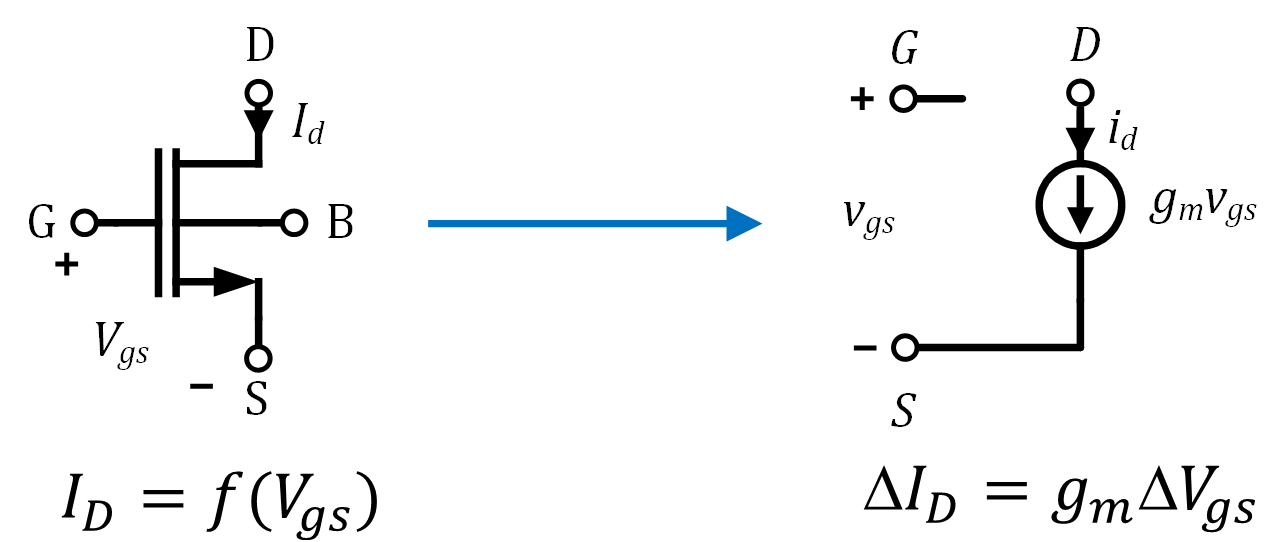
\includegraphics{SS_transconductance.png}
\caption{SS\_transconductance.png}
\end{figure}

    \begin{itemize}
\tightlist
\item
  Instead of having to carry out the linearization process for every new
  circuit we build, we can linearize at the transistor level
\item
  As such, the nonlinear function relating \(I_d\) to \(V_{gs}\) is
  replaced with a linear transconductance term, \(g_m\)
\item
  Transistor linearization allows us to use linear circuit analysis
  techniques (i.e.~Kirchoff's laws) to analyze circuits comprising MOS
  transistors
\end{itemize}

    \hypertarget{linear-transconductance-versus-nonlinear-square-law}{%
\subsubsection{Linear transconductance versus nonlinear square
law}\label{linear-transconductance-versus-nonlinear-square-law}}

    \begin{tcolorbox}[breakable, size=fbox, boxrule=1pt, pad at break*=1mm,colback=cellbackground, colframe=cellborder]
\prompt{In}{incolor}{66}{\boxspacing}
\begin{Verbatim}[commandchars=\\\{\}]
\PY{k}{def} \PY{n+nf}{nmos\PYZus{}iv}\PY{p}{(}\PY{n}{V\PYZus{}gs}\PY{p}{,} \PY{n}{W}\PY{p}{,} \PY{n}{L}\PY{p}{)}\PY{p}{:}
    \PY{n}{u\PYZus{}n} \PY{o}{=} \PY{l+m+mi}{350}                 \PY{c+c1}{\PYZsh{} electron mobility (device parameter)}
    \PY{n}{e\PYZus{}ox} \PY{o}{=} \PY{l+m+mf}{3.9}\PY{o}{*}\PY{l+m+mf}{8.854e\PYZhy{}12}\PY{o}{/}\PY{l+m+mi}{100}\PY{p}{;} \PY{c+c1}{\PYZsh{} relative permittivity}
    \PY{n}{t\PYZus{}ox} \PY{o}{=} \PY{l+m+mf}{9e\PYZhy{}9}\PY{o}{*}\PY{l+m+mi}{100}\PY{p}{;}          \PY{c+c1}{\PYZsh{} oxide thickness}
    \PY{n}{C\PYZus{}ox} \PY{o}{=} \PY{n}{e\PYZus{}ox}\PY{o}{/}\PY{n}{t\PYZus{}ox}          \PY{c+c1}{\PYZsh{} oxide capacitance}
    \PY{n}{V\PYZus{}th} \PY{o}{=} \PY{l+m+mf}{0.7}                \PY{c+c1}{\PYZsh{} threshold voltage (device parameter)}
    
    \PY{n}{I\PYZus{}d} \PY{o}{=} \PY{l+m+mf}{0.5}\PY{o}{*}\PY{n}{u\PYZus{}n}\PY{o}{*}\PY{n}{C\PYZus{}ox}\PY{o}{*}\PY{p}{(}\PY{n}{W}\PY{o}{/}\PY{n}{L}\PY{p}{)}\PY{o}{*}\PY{p}{(}\PY{n}{V\PYZus{}gs} \PY{o}{\PYZhy{}} \PY{n}{V\PYZus{}th}\PY{p}{)}\PY{o}{*}\PY{o}{*}\PY{l+m+mi}{2} 

    \PY{k}{return} \PY{n}{I\PYZus{}d}

\PY{k}{def} \PY{n+nf}{g\PYZus{}m}\PY{p}{(}\PY{n}{V\PYZus{}GS0}\PY{p}{,} \PY{n}{W}\PY{p}{,} \PY{n}{L}\PY{p}{)}\PY{p}{:}
    \PY{n}{V\PYZus{}th} \PY{o}{=} \PY{l+m+mf}{0.7}                \PY{c+c1}{\PYZsh{} threshold voltage (device parameter)}
    \PY{n}{I\PYZus{}D0} \PY{o}{=} \PY{n}{nmos\PYZus{}iv}\PY{p}{(}\PY{n}{V\PYZus{}GS0}\PY{p}{,} \PY{n}{W}\PY{p}{,} \PY{n}{L}\PY{p}{)}
    
    \PY{k}{return} \PY{l+m+mi}{2}\PY{o}{*}\PY{n}{I\PYZus{}D0}\PY{o}{/}\PY{p}{(}\PY{n}{V\PYZus{}GS0} \PY{o}{\PYZhy{}} \PY{n}{V\PYZus{}th}\PY{p}{)}

\PY{k}{def} \PY{n+nf}{gm\PYZus{}line} \PY{p}{(}\PY{n}{V\PYZus{}gs}\PY{p}{,} \PY{n}{W}\PY{p}{,} \PY{n}{L}\PY{p}{,} \PY{n}{V\PYZus{}GS0}\PY{p}{,} \PY{n}{I\PYZus{}D0}\PY{p}{)}\PY{p}{:}
    \PY{k}{return} \PY{n}{g\PYZus{}m}\PY{p}{(}\PY{n}{V\PYZus{}GS0}\PY{p}{,} \PY{n}{W}\PY{p}{,} \PY{n}{L}\PY{p}{)}\PY{o}{*}\PY{p}{(}\PY{n}{V\PYZus{}gs} \PY{o}{\PYZhy{}} \PY{n}{V\PYZus{}GS0}\PY{p}{)} \PY{o}{+} \PY{n}{I\PYZus{}D0}

\PY{k}{def} \PY{n+nf}{plot\PYZus{}gm}\PY{p}{(}\PY{n}{V\PYZus{}gs}\PY{p}{,} \PY{n}{W}\PY{p}{,} \PY{n}{L}\PY{p}{,} \PY{n}{V\PYZus{}GS1}\PY{p}{,} \PY{n}{V\PYZus{}gs\PYZus{}range}\PY{p}{)}\PY{p}{:}
    \PY{n}{fig}\PY{p}{,} \PY{n}{ax} \PY{o}{=} \PY{n}{plt}\PY{o}{.}\PY{n}{subplots}\PY{p}{(}\PY{n}{figsize}\PY{o}{=}\PY{p}{(}\PY{l+m+mf}{10.0}\PY{p}{,}\PY{l+m+mf}{7.5}\PY{p}{)}\PY{p}{)}
    \PY{n}{ax}\PY{o}{.}\PY{n}{plot}\PY{p}{(}\PY{n}{V\PYZus{}gs}\PY{p}{,} \PY{l+m+mf}{1e3}\PY{o}{*}\PY{n}{nmos\PYZus{}iv}\PY{p}{(}\PY{n}{V\PYZus{}gs}\PY{p}{,} \PY{n}{W}\PY{p}{,} \PY{n}{L}\PY{p}{)}\PY{p}{,} 
            \PY{n}{label}\PY{o}{=}\PY{l+s+sa}{r}\PY{l+s+s1}{\PYZsq{}}\PY{l+s+s1}{\PYZdl{}}\PY{l+s+s1}{\PYZbs{}}\PY{l+s+s1}{frac}\PY{l+s+si}{\PYZob{}1\PYZcb{}}\PY{l+s+si}{\PYZob{}2\PYZcb{}}\PY{l+s+s1}{\PYZbs{}}\PY{l+s+s1}{mu C\PYZus{}}\PY{l+s+si}{\PYZob{}ox\PYZcb{}}\PY{l+s+s1}{\PYZbs{}}\PY{l+s+s1}{frac}\PY{l+s+si}{\PYZob{}W\PYZcb{}}\PY{l+s+si}{\PYZob{}L\PYZcb{}}\PY{l+s+s1}{(V\PYZus{}}\PY{l+s+si}{\PYZob{}gs\PYZcb{}}\PY{l+s+s1}{\PYZhy{}V\PYZus{}}\PY{l+s+si}{\PYZob{}th\PYZcb{}}\PY{l+s+s1}{)\PYZca{}2\PYZdl{}}\PY{l+s+s1}{\PYZsq{}}\PY{p}{)}
    \PY{n}{I\PYZus{}D1} \PY{o}{=} \PY{n}{nmos\PYZus{}iv}\PY{p}{(}\PY{n}{V\PYZus{}GS1}\PY{p}{,} \PY{n}{W}\PY{p}{,} \PY{n}{L}\PY{p}{)}
    \PY{n}{ax}\PY{o}{.}\PY{n}{scatter}\PY{p}{(}\PY{n}{V\PYZus{}GS1}\PY{p}{,} \PY{l+m+mf}{1e3}\PY{o}{*}\PY{n}{I\PYZus{}D1}\PY{p}{,} \PY{n}{color}\PY{o}{=}\PY{l+s+s1}{\PYZsq{}}\PY{l+s+s1}{C3}\PY{l+s+s1}{\PYZsq{}}\PY{p}{,}\PY{n}{s}\PY{o}{=}\PY{l+m+mi}{10}\PY{p}{)}
    \PY{n}{ax}\PY{o}{.}\PY{n}{plot}\PY{p}{(}\PY{n}{V\PYZus{}gs\PYZus{}range}\PY{p}{,} \PY{l+m+mf}{1e3}\PY{o}{*}\PY{n}{gm\PYZus{}line}\PY{p}{(}\PY{n}{V\PYZus{}gs\PYZus{}range}\PY{p}{,} \PY{n}{W}\PY{p}{,} \PY{n}{L}\PY{p}{,} \PY{n}{V\PYZus{}GS1}\PY{p}{,} \PY{n}{I\PYZus{}D1}\PY{p}{)}\PY{p}{,} 
            \PY{l+s+s1}{\PYZsq{}}\PY{l+s+s1}{C3\PYZhy{}\PYZhy{}}\PY{l+s+s1}{\PYZsq{}}\PY{p}{,} \PY{n}{linewidth}\PY{o}{=}\PY{l+m+mi}{2}\PY{p}{,} \PY{n}{label}\PY{o}{=}\PY{l+s+sa}{r}\PY{l+s+s1}{\PYZsq{}}\PY{l+s+s1}{\PYZdl{}g\PYZus{}mV\PYZus{}}\PY{l+s+si}{\PYZob{}gs\PYZcb{}}\PY{l+s+s1}{\PYZdl{}}\PY{l+s+s1}{\PYZsq{}}\PY{p}{)}
    \PY{n}{ax}\PY{o}{.}\PY{n}{set\PYZus{}xlabel}\PY{p}{(}\PY{l+s+sa}{r}\PY{l+s+s1}{\PYZsq{}}\PY{l+s+s1}{\PYZdl{}V\PYZus{}}\PY{l+s+si}{\PYZob{}gs\PYZcb{}}\PY{l+s+s1}{ [V]\PYZdl{}}\PY{l+s+s1}{\PYZsq{}}\PY{p}{)}
    \PY{n}{ax}\PY{o}{.}\PY{n}{set\PYZus{}ylabel}\PY{p}{(}\PY{l+s+sa}{r}\PY{l+s+s1}{\PYZsq{}}\PY{l+s+s1}{\PYZdl{}I\PYZus{}}\PY{l+s+si}{\PYZob{}D\PYZcb{}}\PY{l+s+s1}{ [mA]\PYZdl{}}\PY{l+s+s1}{\PYZsq{}}\PY{p}{)}
    \PY{n}{ax}\PY{o}{.}\PY{n}{grid}\PY{p}{(}\PY{p}{)}
    \PY{n}{ax}\PY{o}{.}\PY{n}{legend}\PY{p}{(}\PY{p}{)}
\end{Verbatim}
\end{tcolorbox}

    \begin{tcolorbox}[breakable, size=fbox, boxrule=1pt, pad at break*=1mm,colback=cellbackground, colframe=cellborder]
\prompt{In}{incolor}{74}{\boxspacing}
\begin{Verbatim}[commandchars=\\\{\}]
\PY{n}{V\PYZus{}gs} \PY{o}{=} \PY{n}{np}\PY{o}{.}\PY{n}{linspace}\PY{p}{(}\PY{l+m+mf}{0.7}\PY{p}{,}\PY{l+m+mi}{1}\PY{p}{,}\PY{n}{num}\PY{o}{=}\PY{l+m+mi}{300}\PY{p}{)}
\PY{n}{V\PYZus{}GS0} \PY{o}{=} \PY{l+m+mf}{0.9}
\PY{n}{V\PYZus{}gs\PYZus{}range} \PY{o}{=} \PY{n}{np}\PY{o}{.}\PY{n}{linspace}\PY{p}{(}\PY{n}{V\PYZus{}GS0}\PY{o}{\PYZhy{}}\PY{l+m+mf}{0.05}\PY{p}{,} \PY{n}{V\PYZus{}GS0}\PY{o}{+}\PY{l+m+mf}{0.05}\PY{p}{,} \PY{l+m+mi}{10}\PY{p}{)}
\PY{n}{plot\PYZus{}gm}\PY{p}{(}\PY{n}{V\PYZus{}gs}\PY{p}{,} \PY{l+m+mi}{1000}\PY{p}{,} \PY{l+m+mi}{1}\PY{p}{,} \PY{n}{V\PYZus{}GS0}\PY{p}{,} \PY{n}{V\PYZus{}gs\PYZus{}range}\PY{p}{)}
\end{Verbatim}
\end{tcolorbox}

    \begin{center}
    \adjustimage{max size={0.9\linewidth}{0.9\paperheight}}{output_76_0.png}
    \end{center}
    { \hspace*{\fill} \\}
    
    \begin{itemize}
\tightlist
\item
  In the vicinity of the linearization, or ``DC operating'' point, the
  linear model well-approximates the square law
\item
  As \(V_{gs}\) becomes much less or greater than \(V_{GS0}\), a
  significant error results in using the linear model
\item
  For this reason, \(g_m\) is used exclusively as a ``small-signal''
  approximation for the transistor behavior
\end{itemize}

    \hypertarget{saturation-transconductance}{%
\subsection{Saturation
transconductance}\label{saturation-transconductance}}

    \begin{itemize}
\tightlist
\item
  Transconductance is defined as the derivative of drain current with
  respect to gate-source voltage
\end{itemize}

\begin{equation}
g_m = \dfrac{\partial I_d}{\partial V_{gs}}\bigg\rvert_{I_d = I_{D0}} = \dfrac{\partial}{\partial V_{gs}} \dfrac{1}{2}\mu C_{ox} \dfrac{W}{L} (V_{gs} - V_{th})^2 \bigg\rvert_{V_{gs} = V_{GS0}}= \mu C_{ox} \left(\dfrac{W}{L} \right) (V_{GS0} - V_{th})
\end{equation}

\begin{itemize}
\tightlist
\item
  In saturation, this can be expressed as
\end{itemize}

\begin{equation}
g_m = \dfrac{2I_{D0}}{(V_{GS0} - V_{th})} = \dfrac{2I_{D0}}{V_{OV}}
\end{equation}

\begin{itemize}
\tightlist
\item
  Importantly, for a constant overdrive \(g_m\) is linearly dependent on
  \(I_{D0}\)
\end{itemize}

    \hypertarget{dependence-of-id-on-vds}{%
\subsection{Dependence of Id on Vds}\label{dependence-of-id-on-vds}}

    \begin{figure}
\centering
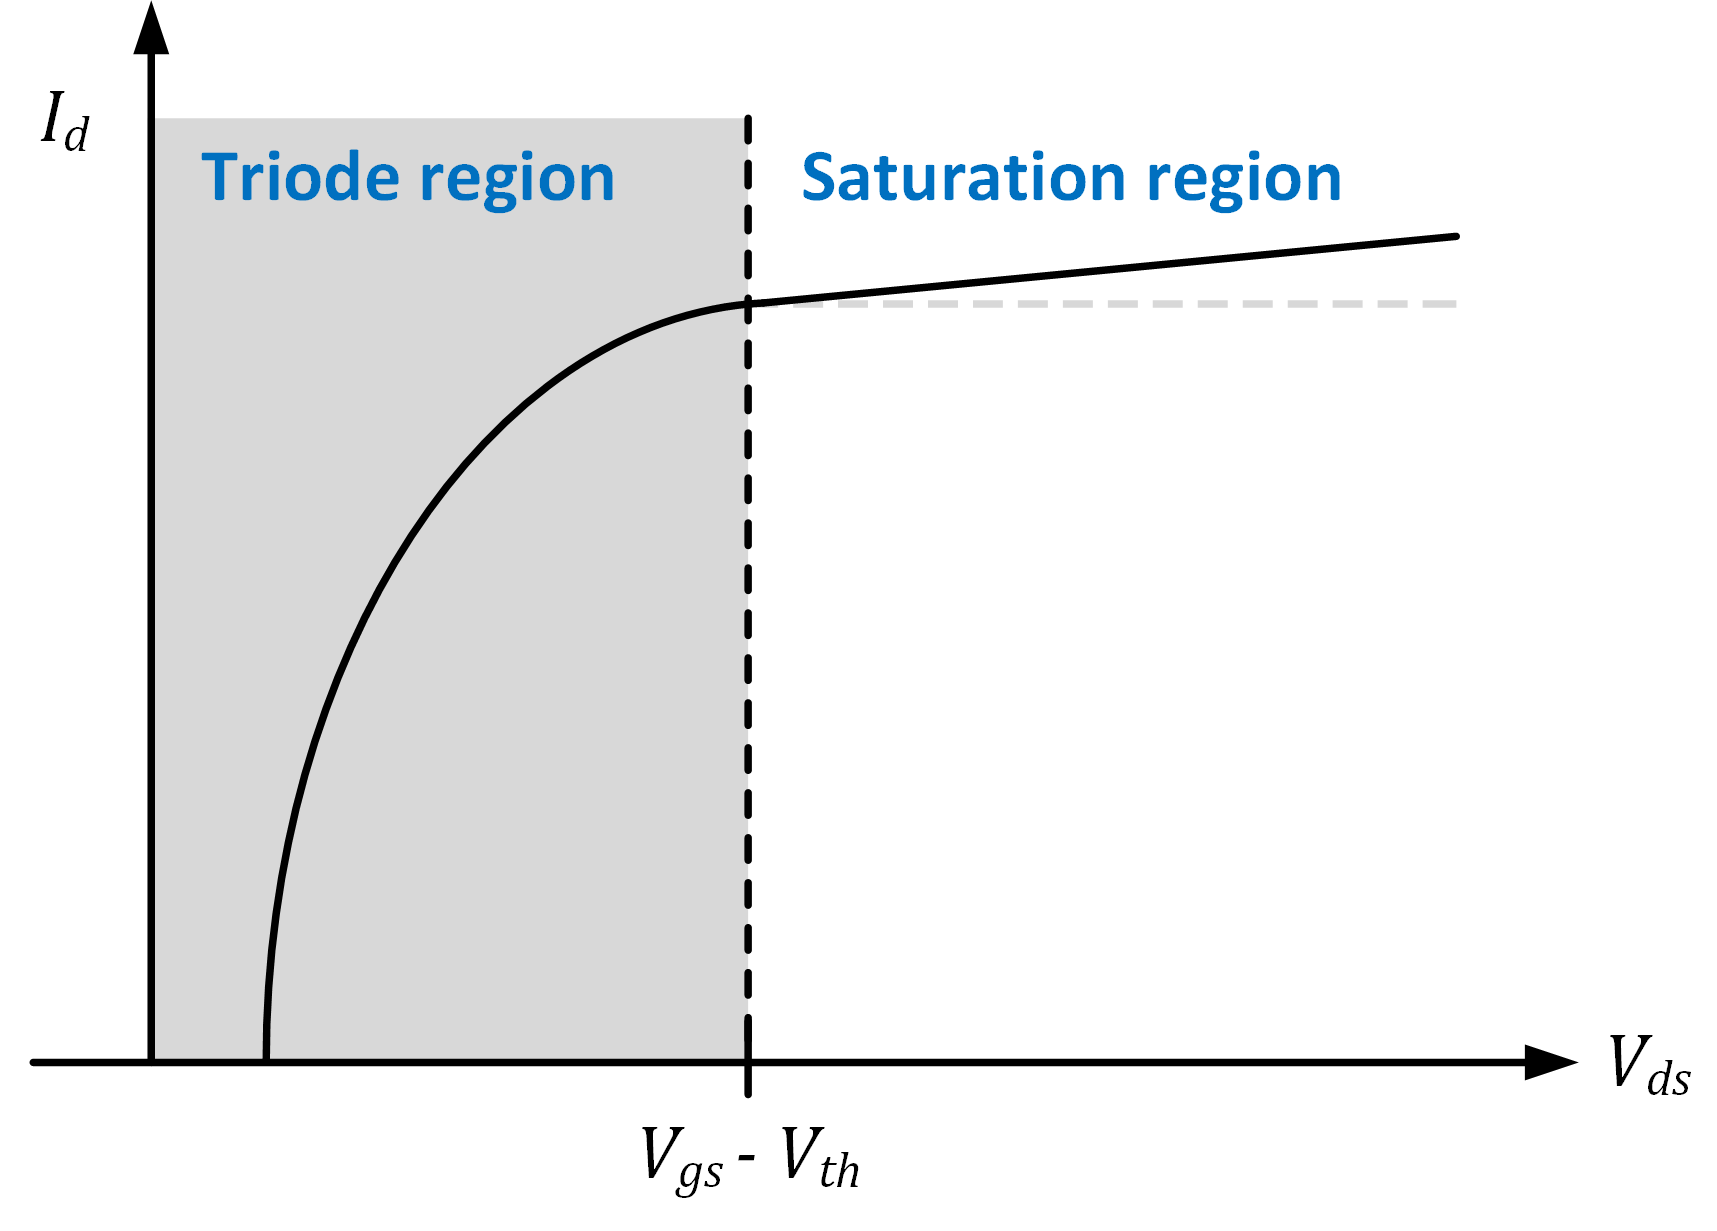
\includegraphics{MOS_regions.png}
\caption{MOS\_regions.png}
\end{figure}

    \begin{itemize}
\tightlist
\item
  If we sweep \(V_{ds}\) of a real transistor, we see a small dependence
  of \(I_d\) on \(V_{ds}\)
\item
  The effect is analogous to the Early effect in BJTs
\item
  The variation of \(I_d\) with \(V_{ds}\) is largely due to a decrease
  in the effective channel length, resulting from the high electric
  field at the drain
\item
  This effect is typically referred to as ``channel-length modulation''
\end{itemize}

    \hypertarget{channel-length-modulation}{%
\subsection{Channel-length modulation}\label{channel-length-modulation}}

    \begin{figure}
\centering
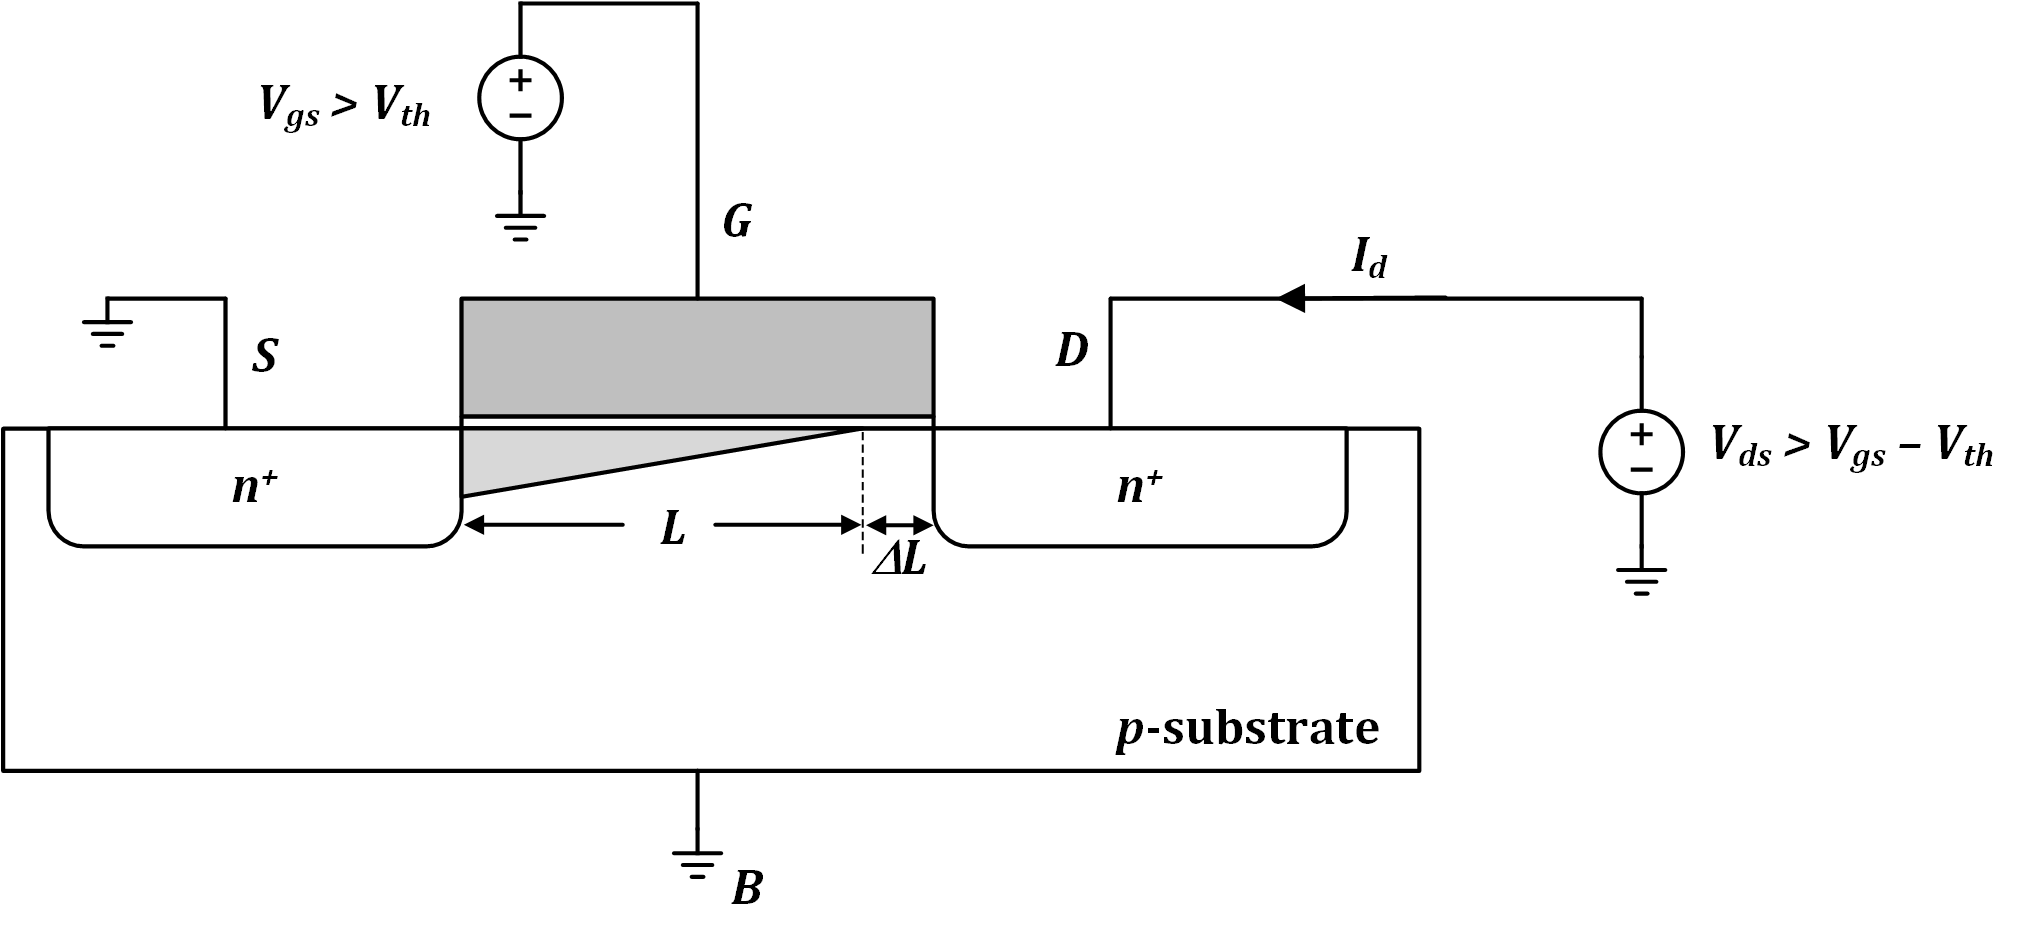
\includegraphics{channel_length_modulation.png}
\caption{channel\_length\_modulation.png}
\end{figure}

    \begin{itemize}
\tightlist
\item
  As \(V_{ds}\) increases, the high \(E\)-field region close to the
  drain grows, decreasing the effective channel length
\item
  The reduced channel length increases the drain current, resulting in a
  positive slope of \(I_d\) vs \(V_{ds}\)
\item
  The effect is more pronounced for shorter gate lengths, due to the
  larger ratio \(\Delta L / L\)
\end{itemize}

    \hypertarget{modified-square-law-expression}{%
\subsection{Modified square-law
expression}\label{modified-square-law-expression}}

    \begin{itemize}
\tightlist
\item
  Finite slope of drain current with repsect to \(V_{ds}\) is typically
  attributed to channel-length modulation
\item
  However, this is actually the result of a combination of a number of
  physical effects (DIBL, SCBE, \ldots)
\item
  A simple model that assumes a linear increase in \(I_d\) with
  \(V_{ds}\) is generally used to model MOS behavior, where the
  combination of effects is lumped into a single parameter, \(\lambda\),
  inversely proportional to channel length \(L\)
  (\(\lambda \propto 1/L\))
\item
  The drain current expression is modified as
\end{itemize}

\begin{equation}
\boxed{I_d = \dfrac{1}{2}\mu\cdot C_{ox} \cdot \dfrac{W}{L}(V_{gs}-V_{th})^2 (1+\lambda V_{ds})}
\end{equation}

    \hypertarget{i-v-characteristic-with-channel-length-modulation}{%
\subsection{I-V characteristic with channel-length
modulation}\label{i-v-characteristic-with-channel-length-modulation}}

    \begin{tcolorbox}[breakable, size=fbox, boxrule=1pt, pad at break*=1mm,colback=cellbackground, colframe=cellborder]
\prompt{In}{incolor}{73}{\boxspacing}
\begin{Verbatim}[commandchars=\\\{\}]
\PY{n}{plot\PYZus{}ID\PYZus{}curves}\PY{p}{(}\PY{n}{V\PYZus{}gs}\PY{p}{,} \PY{n}{V\PYZus{}ds}\PY{p}{,} \PY{l+m+mi}{100}\PY{p}{,} \PY{l+m+mi}{1}\PY{p}{,} \PY{o}{.}\PY{l+m+mi}{05}\PY{p}{)}
\end{Verbatim}
\end{tcolorbox}

    \begin{center}
    \adjustimage{max size={0.9\linewidth}{0.9\paperheight}}{output_89_0.png}
    \end{center}
    { \hspace*{\fill} \\}
    
    \begin{itemize}
\tightlist
\item
  The inclusion of \(\lambda\) in the square-law model results in a
  finite slope of the \(I_d\) vs \(V_{ds}\) curves
\item
  This dependence of \(I_d\) on \(V_{ds}\) is referred to as the
  transistor \emph{output resistance}, which is determined by taking the
  derivative of \(I_d\) with respect to \(V_{ds}\):
\end{itemize}

\begin{equation}
r_o = \left(\dfrac{d}{dV_{ds}}I_d \right)^{-1}\bigg\rvert_{I_d = I_{D0}} =  \dfrac{1}{\lambda \cdot \dfrac{1}{2}\mu\cdot C_{ox} \cdot \dfrac{W}{L}(V_{gs}-V_{th})^2}\bigg\rvert_{V_{gs} = V_{GS0}} = \dfrac{1}{\lambda I_{D0}}
\end{equation}

    \hypertarget{mos-dc-model-intrinsic-gain}{%
\subsection{MOS DC model (intrinsic
gain)}\label{mos-dc-model-intrinsic-gain}}

    \begin{figure}
\centering
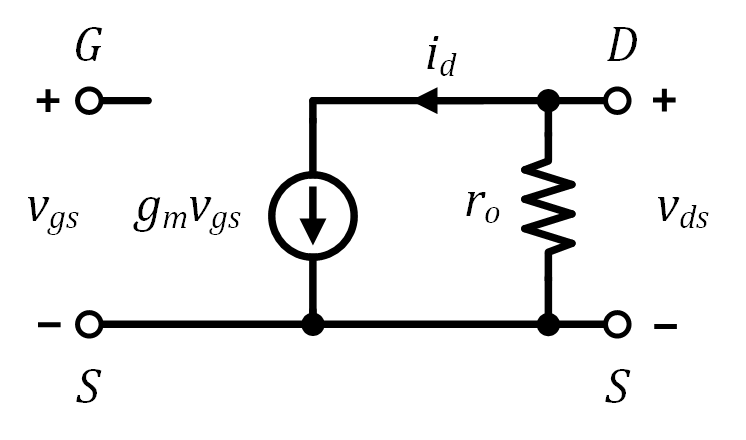
\includegraphics{MOS_intrinsic_gain.png}
\caption{MOS\_intrinsic\_gain.png}
\end{figure}

    \begin{equation}
g_m = \dfrac{2I_{D0}}{V_{OV}}
\end{equation}

\begin{equation}
r_o = \dfrac{1}{g_{ds}} = \dfrac{1}{\lambda I_{D0}}
\end{equation}

\begin{equation}
\left|\dfrac{v_{ds}}{v_{gs}}\right| = \dfrac{g_m}{g_{ds}} = \dfrac{2}{V_{OV}}
\end{equation}

    \begin{itemize}
\tightlist
\item
  The dependence of \(I_d\) on \(V_{ds}\) is modeled as a resistance
  \(r_o\), referred to as the transistor \emph{output impedance}, which
  is linearly dependent on \(I_d\)
\item
  The product \(g_m \cdot r_o\) is called the intrinsic gain of the
  MOSFET, which is, to first order, independent of drain current
\item
  As we will see, intrinsic gain is a fundamental device property that
  affects a number of circuit performance metrics (e.g.~voltage gain of
  an amplifier)
\end{itemize}

    \hypertarget{level-1-nmospmos-spice-models}{%
\subsection{Level 1 NMOS/PMOS SPICE
models}\label{level-1-nmospmos-spice-models}}

    \begin{longtable}[]{@{}crcc@{}}
\toprule
NMOS Model & & &\tabularnewline
\midrule
\endhead
LEVEL = 1 & VTO = 0.7 & GAMMA = 0.45 & PHI = 0.9\tabularnewline
NSUB = 9e+14 & LD = 0.08e-6 & UO = 350 & LAMBDA = 0.1\tabularnewline
TOX = 9e-9 & PB = 0.9 & CJ = 0.56e-3 & CJSW = 0.35e-11\tabularnewline
MJ = 0.45 & MJSW = 0.2 & CGDO = 0.4e-9 & JS = 1.0e-8\tabularnewline
\bottomrule
\end{longtable}

\begin{longtable}[]{@{}crcc@{}}
\toprule
PMOS Model & & &\tabularnewline
\midrule
\endhead
LEVEL = 1 & VTO = -0.8 & GAMMA = 0.4 & PHI = 0.8\tabularnewline
NSUB = 5e+14 & LD = 0.09e-6 & UO = 100 & LAMBDA = 0.2\tabularnewline
TOX = 9e-9 & PB = 0.9 & CJ = 0.94e-3 & CJSW = 0.32e-11\tabularnewline
MJ = 0.5 & MJSW = 0.3 & CGDO = 0.3e-9 & JS = 0.5e-8\tabularnewline
\bottomrule
\end{longtable}

    \hypertarget{comments-on-models}{%
\subsection{Comments on models}\label{comments-on-models}}

    \begin{itemize}
\tightlist
\item
  The model discussed here is often referred to as the ``long-channel''
  or ``square-law'' model
\item
  Although it is intuitively satisfying and readily applied
  analytically, it is grossly inadequate for modeling modern
  ``short-channel'' devices
\item
  To accurately model a wide range of ``second-order'' effects, a
  complex transistor model with many empirical parameters, must be used
\item
  However, the long-channel model is useful for gaining intuition and
  understanding general performance trends
\item
  A rule of thumb is useful here: \textbf{Use the simplest model that is
  accurate enough for the task}
\end{itemize}

    \hypertarget{summary}{%
\subsection{Summary}\label{summary}}

    \begin{itemize}
\tightlist
\item
  Long-channel ``square-law'' model provides an intuitive picture of MOS
  device operation

  \begin{itemize}
  \tightlist
  \item
    \(g_m\) linearly dependent on \(I_d\) if \(V_{gs} - V_{th}\) is
    constant
  \item
    \(r_o\) inversely dependent on \(I_d\)
  \item
    Intrinsic gain \(g_m \cdot r_o\) independent of \(I_d\)
  \end{itemize}
\item
  Small-signal model will be used to design circuits with specific gain
  and impedance characteristics
\end{itemize}


    % Add a bibliography block to the postdoc
    
    
    
\end{document}
